%%%%%%%%%%%%%%%%%%%%%%%%%%%%%%%%%%%%%%%%%%%%%%%%%%%%%%%%%%%%%%%%%%%%%%%%%%%%%%%
% Descripción: Template para la generación de la tesis de la MDIAE
% Autor: 
% Fecha: 20/05/2016
%%%%%%%%%%%%%%%%%%%%%%%%%%%%%%%%%%%%%%%%%%%%%%%%%%%%%%%%%%%%%%%%%%%%%%%%%%%%%%%

%%%%%%%%%%%%%%%%%%%%%%%%%%%%%%%%%%%%%%%%%%%%%%%%%%%%%%%%%%%%%%%%%%%%%%%%%%%%%%%
%%	PARA INSERTAR FIGURAS USAR LA FUNCION PREDEFINIDA \imagen
%%
%%      \imagen{escala}{path imagen}{caption}{referencia}
%%
%% donde:
%% 	* escala: es un valor numérico. Preferentemente usar valores entre 0 y 1.
%%		(ejemplo: 0.2)
%% 	* path: imagen es el directorio relativo donde se encuentra la imagen
%%		(ejemplo: Figures/Logos/conae-logo.png)
%%	* caption: texto de pie de figura.
%%	* referencia: texto que sirve para citar la figura. 
%%		(ejemplo: fig:conaelogo) luego se podrá hacer referencia \ref{fig:conaelogo}
%%%%%%%%%%%%%%%%%%%%%%%%%%%%%%%%%%%%%%%%%%%%%%%%%%%%%%%%%%%%%%%%%%%%%%%%%%%%%%%

%------------------------------------------------------------------------------
% Formato del documento
\documentclass[12pt, a4paper, twoside]{report}

%------------------------------------------------------------------------------
% TEMPLATE MDIAE (ACÁ SE ENCUETRAN LAS CUSTOMIZACIONES)
% Remitirse al archivo mdiaedoc.sty

\usepackage{mdiaedoc}


%Configuración de los márgenes
\usepackage[top=3cm, bottom=3cm, left=2.5cm, right=1.5cm]{geometry}
%\newwatermark[allpages,color=lightgray!50,angle=45,scale=3,xpos=0,ypos=0]{PRELIMINAR}
%
%------------------------------------------------------------------------------
% Esto no se usa (YA ESTA DEFINIDO EN EL TEMPLATE)
%\usepackage{setspace}

%%%%%%%%%%%%%%%%%%%%%%%%%%%%%%%%%%%%%%%%%%%%%%%%%%%%%%%%%%%%%%%%%%%%%%%%%%%%%%%
% COMIENZO DEL DOCUMENTO
%%%%%%%%%%%%%%%%%%%%%%%%%%%%%%%%%%%%%%%%%%%%%%%%%%%%%%%%%%%%%%%%%%%%%%%%%%%%%%%
\begin{document}

\makeatletter
\author{M. Cecilia Valenti}
\makeatother

%------------------------------------------------------------------------------
% PORTADA
\portadatesis{ARxCODE\\Prototipo de software para el An\'alisis de Riesgo por Colisi\'on con Desechos Espaciales.}{M. Cecilia Valenti.}{UNIVERSIDAD NACIONAL DE LA MATANZA}{}{}{Marcelo Colazo}{Comisi\'on Nacional de Actividades Espaciales (CONAE)}{Dra. Alicia Mon}{Universidad Nacional de la Matanza (UNLaM)}

%------------------------------------------------------------------------------
%EN CASO DE TENER UN ASESOR CIENTIFICO, DESCOMENTAR LO SIGUIENTE 
% \begin{center}
% \normalsize CO-DIRECTORA:\\
% \normalsize \textit{\textbf{Dra. Alicia Mon}}\\
% \end{center}

%------------------------------------------------------------------------------
% COMPLETAR CON LICENCIA CREATIVE COMMONS SEGÚN CORRESPONDA
%\begin{center}
%%%%% Ejemplo %%%%%%
%\begin{figure}[H]
%    \centering
%    \includegraphics[width=3cm, keepaspectratio=true]{imagenes/Logos/creativecommons.png}
%\end{figure}
%\vspace*{-0.5cm}
%Esta obra está bajo una \href{http://creativecommons.org/licenses/by-sa/2.5/ar/}{Licencia Creative Commons Atribución-CompartirIgual 2.5 Argentina.}
%\end{center}

\pagenumbering{gobble}

% \chapter*{Abstract}
\label{chap:abstract}

\textbf{Keywords:}
\chapter*{Resumen}
\label{chap:resumen}


%%%% Texto (no menos de 200 palabras)

\textbf{Palabras clave:}
\chapter*{Agradecimientos}
\label{chap:agradecimientos}

En primer lugar, agradezco a mi director Marcelo Colazo, que dirigi\'o este trabajo y desde hace ya varios a\~nos me acompa\~na y me ayuda en las distintas oportunidades que van surgiendo para mi desarrollo profesional. 

Agradezco tambi\'en a Alicia Mon, mi codirectora y a los jurados: Jos\'e L. Roca, Walkiria Shulz y Livio Gratton por su tiempo y dedicaci\'on en la revisi\'on detallada del trabajo. 

Al director del Instituto M. Gulich, Leonardo De Ferraris, al director de la MDIAE Carlos Barrientos, al Dr. Jorge Ierache y a todas las autoridades, docentes y personal administrativo tanto de la UFS de CONAE como de la UNLaM, que trabajaron para hacer posible esta maestr\'ia.\\


A t\'itulo personal, agradezco a mis compa\~neros de cursada y los amigos que estuvieron cerca en esta etapa. Agradezco profundamente a mi familia por el apoyo incondicional siempre y a Soligo, mi compa\~nero de mates y de vida.\\


Por \'ultimo, agradezco a todo el pueblo argentino que ha financiado mi formaci\'on de grado en la universidad pública de La Plata y esta maestr\'ia entre la universidad p\'ublica de la Matanza y la CONAE. 





 %% OPCIONAL

\tabladecontenidos

\chapter*{Lista de acrónimos}
\label{chap:acronimos}

\begin{acronym}[ARxCODE]
\acro{CONAE}{Comisi\'on Nacional de Actividades Espaciales}
\acro{ARxCODE}{An\'alisis de Riesgo por Colisi'on con Desechos Espaciales}
\acro{CDM}{Conjunction Data Message}
\acro{TLE}{Two-Line elements}
\acro{SGP4}{Simplified General Perturbations model}
\acro{JSpOC}{Joint Space Operations Center}
\acro{NORAD}{North American Aerospace Defense Command}
\acro{PoC}{Probability of Collision}
\acro{TCA}{Time of Closest Approach}
\acro{ESA}{European Space Agency}
\acro{NASA}{National Aeronautics and Space Administration}
\acro{ISS}{International Space Station}
\acro{RMM}{Risk Mitigation Maneuver}
\acro{COPUOS}{Committee of the Peacefull Uses of Outer Space (ONU)}
\acro{IADC}{Inter-Agency Space Debris Coordination Commitee}
\acro{CCSDS}{Consultative Committee for Space Data Systems}
\end{acronym}



%------------------------------------------------------------------------------
% Numeración arábiga a partir de este punto
\pagenumbering{arabic}
\setcounter{page}{1}

\chapter{Introducción}
\label{chap:introduccion}


\section{Los desechos espaciales}

El comienzo de la era satelital en el a\~no 1957 con la puesta en \'orbita del sat\'elite ruso Sputnik signific\'o la conquista de un nuevo espacio y un cambio de paradigma en lo que respecta a las tecnolog\'ias para las comunicaciones, los estudios de nuestro planeta, el sistema solar, las formas de navegar, de geoposicionarse y el intercambio de informaci\'on. Desde entonces el ambiente espacial cada vez suma m\'as colonos (Fig. \ref{fig:cantidad2014}).\\

Las experiencias de las primeras misiones aportaron mucho conocimiento de este entorno con caracter\'isticas muy distintas a las de la superficie de la Tierra y permitieron ir mejorando las t\'ecnicas y los materiales para que los sat\'elites cumplieran sus objetivos sin mayores inconvenientes.\\
Sin embargo, un hecho poco predicho o abordado empez\'o a ocupar prioridad en las dos \'ultimas d\'ecadas: los {\it{desechos espaciales}}.\\

{\bf{Definici\'on:}}{\it{ Son Desechos Espaciales todos los objetos construidos por el hombre, incluyendo fragmentos o partes de los mismos, que orbitan la Tierra o reingresan a la atm\'osfera y no son funcionales, es decir, han perdido su capacidad operativa.}} \citep{iadcguide}\\

La disponibilidad del espacio parec\'ia ilimitada, y los primeros a\~nos no se ten\'ian consideraciones respecto a los objetos que all\'i se depositaban, o se desprend\'ian de los cohetes y las misiones. Pero con el correr del tiempo, ciertas regiones del espacio cobraron inter\' es estrat\'egico, y la superpoblaci\'on en dichas zonas no tard\'o en mostrar complicaciones.\\

Los desechos representan hoy el mayor porcentaje de los objetos que orbitan la Tierra y los estudios de su proliferaci\'on, indican que, de no existir planes de acci\'on para subsanar la situaci\'on, el efecto de las colisiones en cascada transformar\'a el ambiente espacial en un lugar inhabitable para cualquier misi\'on.\\

La primera colisi\'on confirmada y claramente registrada entre una misi\'on operativa y un desecho, ocurri\'o el 24 de Julio de 1996, cuando el sat\'elite franc\'es Cerise (95-033B) fue embestido por un fragmento (86-019RF), remanente de la explosi\'on de la \'ultima etapa del cohete Ariane-1 H-10, ocurrida el 13 de noviembre de 1986; nueve meses despu\'es de inyectar en \'orbita al sat\'elite SPOT-1. La reconstrucci\'on de la situaci\'on luego de la colisi\'on, coincide plenamente con una p\'erdida de la actitud del Cerise que fue registrada en los datos hist\'oricos abordo. \citep{KlinkradChapter8}\\

Este accidente fue un disparador en lo que respecta al estudio de los desechos espaciales y las colisiones. Las estad\'isticas de la base de datos de Scopus \footnote{https://www.scopus.com/}, indican que las investigaciones respecto a la tem\'atica de desechos espaciales en general muestran un continuo crecimiento, ver figura \ref{fig:scopusSD}.\\
Lo mismo ocurre en la tem\'atica de colisiones (figura \ref{fig:scopusCA}), destac\'andose el gran escal\'on a partir del a\~no 1993 (colisi\'on del sat\'elite Cerise), un pico a partir del a\~no 1998, probablemente vinculado al lanzamiento de la estaci\'on espacial internacional o \ac{ISS}, y luego un notorio crecimiento a partir del a\~no 2007, vinculado a dos sucesos: la destrucci\'on intencional de China de uno de sus sat\'elites en una prueba misil\'istica y la colisi\'on catastr\'ofica accidental entre el sat\'elite ruso KOSMOS 2251, fuera de servicio y el sat\'elite IRIDIUM 33, operativo, de la constelaci\'on de IRIDIUM, en el a\~no 2009.\\


\begin{figure}[!h]
\centering
  \textbf{Publicaciones sobre Desechos Espaciales (Scopus)}\par\medskip
    \fbox{\includegraphics[width=0.8\columnwidth, keepaspectratio]{imagenes/scopusSD}}
    \caption[Desechos Espaciales seg\'un Scopus]{Estad\'istica de las investigaciones realizadas en el \'area de desechos espaciales ({\it{Space Debris}}) de acuerdo a la base de datos de Scopus.}
    \label{fig:scopusSD}
\end{figure}

\begin{figure}[!h]
\centering
   \textbf{Publicaciones sobre Colisiones (Scopus)}\par\medskip
    \fbox{\includegraphics[width=0.7\columnwidth, keepaspectratio]{imagenes/scopusCA}}
    \caption[Riesgos de Colisi\'on seg\'un Scopus]{Estad\'istica de las investigaciones realizadas en el \'area de riesgos de colisi\'on {\it{Collision Avoidance}} de acuerdo a la base de datos de Scopus.}
    \label{fig:scopusCA}
\end{figure} 

\subsection*{Distintos abordajes para el estudio de los desechos espaciales}
Existen distintos estudios respecto a la problem\'atica de los desechos espaciales. La \ac{NASA} propone una clasificaci\'on general seg\'un sean estudios de: modelado, rastreo, protecci\'on, mitigaci\'on, reparaci\'on o reingreso.\\
\begin{itemize}
%\setlength{\itemsep}{0pt}
\item {\bf{Modelado:}} Consiste en el desarrollo y la actualizaci\'on de los modelos orbitales de los desechos, para describir y caracterizar el ambiente actual y la proyecci\'on futura.\\
\item {\bf{Rastreo:}} Mediciones que se hacen con radares y telescopios \'opticos desde tierra, y tambi\'en con telescopios espaciales.\\
\item {\bf{Protecci\'on:}} Estudios hechos en impactos de alta velocidad para el desarrollo de nuevos materiales y dise\~nos que ofrezcan una mayor protecci\'on.\\
\item {\bf{Mitigaci\'on:}} Planifiaci\'on de estrategias para reducir la generaci\'on de nuevos desechos. Generaci\'on de documentaci\'on  de buenas pr\'acticas, est\'andares y promoci\'on de acuerdos internacionales.\\
\item {\bf{Reparaci\'on:}} Dise\~no de misiones con el \'unico objetivo de actuar sobre los desechos a fin de reducir el n\'umero de objetos inactivos en \'orbita.\\
\item {\bf{Reingreso:}} Identificaci\'on de los reingresos no controlados, para hacer an\'alisis sobre las zonas de posibles impactos en Tierra y la planificaci\'on de reingresos controlados.\\
\end{itemize}

Organismos como el Centro Principal de Inteligencia Espacial Ruso, el Departamento de Defensa Norteamericano, la NASA y la \ac{ESA}, han desarrollado tanto modelos de evoluci\'on como de ingenier\'ia, y mantienen cat\'alogos actualizados con las trayectorias de aquellos objetos cuyo tama\~no permite detectarlos con instrumentos de rastreo en Tierra.\\

Los modelos de evoluci\'on muestran la configuraci\'on actual y proyecciones de configuraciones futuras del ambiente espacial incluyendo todos los objetos que orbitan la Tierra.\\

Los modelos de ingenier\'ia se enfocan en distintas pruebas de laboratorio o de misiones espec\'ificas en \'orbita, que analizan la respuesta de los materiales cuando se exponen a impactos con fragmentos de distinto tipo, particularmente en aquellos de tama\~nos muy chicos pero que colisionan a velocidades del orden de diez kil\'ometros por segundo.\\

En este trabajo nos enfocamos en el an\'alisis de las situaciones de riesgo de colisi\'on, dentro del marco de la {\it{mitigaci\'on}}, para las misiones y los desechos que se ubican en las  \ac{LEO}, u \'orbitas bajas.\\

\subsection*{El entorno de los desechos espaciales: presente y futuro}
Seg\'un los informes de la \ac{ESA} \citep{esaSD}, desde 1957 hasta la actualidad, 5250 lanzamientos han poblado el ambiente espacial con casi 23000 objetos de los cuales, s\'olo cerca de 1200 son sat\'elites operativos.\\

El \ac{IADC}, clasifica los desechos seg\'un sean: objetos relacionados a alguna misi\'on, Fragmentos, o cohetes y objetos que ya finalizaron su misi\'on. Ver tabla \ref{tab:desechosIADC}.\\

\begin{table}[h]\renewcommand{\arraystretch}{1.3}
\centering
\resizebox{17cm}{!}{
\begin{tabular}[c]{|l|l|l|}
\hline 
\rowcolor{lightgray}
\bf{Clasificaci\'on}  &    \bf{Causas} & \bf{Recomendaciones del IADC}\\
\hline
\multirow{ 2}{*}{Objetos relacionados a una misi\'on} &   Liberados intencionalmente& Dise\~nos que reduzcan la liberaci\'on de desechos\\
&Liberados sin intenci\'on& Dise\~nos robustos\\
\hline
\multirow{ 4}{*}{Fragmentos}& Destrucci\'on intencional & Evitar destrucciones intencionales.\\
& Fragmentaciones durante las operaciones & Aseguramiento de la misi\'on.\\
& Fragmentaciones ya finalizada la misi\'on & Reducci\'on de estas situaciones en el dise\~no.\\
& \cellcolor{blue!25}{Colisiones en \'orbita} & Planificaci\'on de maniobras evasivas por riesgo\\
&&de colisi\'on. Protecci\'on.\\
\hline
Objetos que ya finalizaron & Maniobras de disposal inadecuadas &Maniobras de reingreso\\
su misi\'on y cohetes && \\
\hline
\end{tabular} }
\caption[Clasificaci\'on de Desechos seg\'un la IADC]{Clasificaci\'on de Desechos, las causas y las recomendaciones adaptado de la gu\'ia de recomendaciones del \cite{iadcguide}}
\label{tab:desechosIADC}
\end{table}


De a acuerdo a una publicaci\'on de la \cite{ODQNum}, hasta el 04 de Abril de 2017, se contabilizaron $18347$ objetos catalogados (Ver tabla \ref{tab:objpais}). Clasificados seg\'un sean: cargas \'utiles ({\it{payloads}}), cohetes ({\it{rocket bodies}}), desechos de misi\'on ({\it{mission-related bodies}}), desechos an\'omalos ({\it{anomalous debris}}) o desechos de fragmentaci\'on ({\it{breakup debris}}); ver figura \ref{fig:catxtipo}.\\

\begin{table}
 \centering
 \begin{tabular}{|l|c|c|c|}
  \hline \hline
  \rowcolor{lightgray}
  \bf{Pa\'is}  &    \bf{Cargas \'Utiles} & \bf{Cohetes y Desechos} & TOTAL\\
  \hline \hline
  China & 235 & 3566&3801\\
  \hline
  CIS & 1508&4993&6501\\
  \hline
  ESA &74&60&134\\
  \hline
  Francia & 62&470&532\\
  \hline
  India & 79 & 113 & 192\\
  \hline
  Jap\'on & 162 & 94 & 256\\
  \hline
  USA & 1513 & 4504 & 6017\\
  \hline
  Otros & 801 & 113 & 914 \\
  \hline\hline
  \rowcolor{lightgray}
  TOTAL & 4434 & 13913 & 18347 \\
  \hline\hline
 \end{tabular}
 \caption[Objetos en \'Orbita al 4 de Abril de 2017.]{Objetos en \'Orbita al 4 de Abril de 2017. Adatado de \cite{ODQN}}
 \label{tab:objpais}
\end{table}

\begin{figure}[!h]
\centering
    \fbox{\includegraphics[width=0.7\columnwidth, keepaspectratio]{imagenes/clasificacion2016}}
    \caption[Objetos en \'Orbita seg\'un NASA.]{Porcentaje de Objetos en \'Orbita seg\'un la clasificaci\'on de NASA. Extra\'ido de \cite{ODQN}}
    \label{fig:catxtipo}
\end{figure}

Otra clasificaci\'on podr\'ia ser en funci\'on de la distancia a la superficie de la Tierra, ya que la distribuci\'on no es homog\'enea. La relaci\'on entre la densidad de objetos y la altura a la que se encuentran, señala que existen regiones m\'as comprometidas.
Las \'orbitas bajas o \ac{LEO} con un rango de alturas entre los 500 y los 2000 kil\'ometros, son las m\'as superpobladas y contienen casi el 70 \% de todos los objetos catalogados. 
Cabe destacar que en esta regi\'on se ubican las misiones de la serie SAC de la CONAE, las misiones futuras SAOCOM Y SABIAMAR. Ver figura \ref{fig:Dvsaltura}.\\

\begin{figure}[!h]
  \centering
  \includegraphics[width=0.9\textwidth]{imagenes/SDvsaltura2011CONAE}
  \caption[Distribuci\'on de objetos en funci\'on del semieje mayor.]{Distribuci\'on de objetos en funci\'on del semieje mayor en la regi\'on LEO. Adapatado de \citep{Klinkrad}. Se agregan en color azul las posiciones de las misiones de CONAE ya puestas en \'orbita (serie SAC) y en color naranja las posiciones de las futuras misiones SAOCOM y SABIAMAR}
  \label{fig:Dvsaltura}
\end{figure}

Si se mira hacia el futuro, las predicciones no son alentadoras. Si bien, los acuerdos internacionales en relaci\'on a acciones para reducir la proliferaci\'on de desechos avanzan y muestran buenos resultados, los proyectos de nuevas misiones tienden a aumentar el n\'umero de objetos, sobre todo en las \'orbitas bajas. Para estas \'orbitas las colisiones pasar\'ian a ser las principales generadoras de desechos.\\

En un reporte t\'ecnico publicado por la NASA \citep{karacalioglu2016impact}, se eval\'uan las nuevas tendencias de la industria satelital y se analiza el futuro panorama del entorno espacial en las \'orbitas bajas, en funci\'on de los lanzamientos planificados y las misiones anunciadas, Fig. \ref{fig:satxlanz}.\\

En los \'ultimos a\~nos se ha incrementado el n\'umero de agencias o empresas que se dedican al desarrollo espacial. El nuevo paradigma de constelaciones de peque\~nos sat\'elites, sistemas distribuidos o arquitecturas fragmentadas en reemplazo de los grandes y costosos sat\'elites tradicionales, ha permitido la democratizaci\'on del espacio, facilit\'andole el acceso a m\'as agencias y empresas.\\ 
Un claro ejemplo son las constelaciones para comunicaciones anunciadas por OneWeb y SpaceX, que proyectan lanzar del orden de 600 sat\'elites cada una para fines del 2019.\\

\begin{figure}[!h]
  \centering
  \includegraphics[width=0.7\textwidth]{imagenes/satelxlanz}
  \caption[Proyecci\'on de Sat\'elites 2016-2030]{Proyecci\'on de Sat\'elites 2016-2030. Extra\'ido de \citep{karacalioglu2016impact}}
  \label{fig:satxlanz}
\end{figure}

Estas futuras misiones, no s\'olo generan un aumento en la poblaci\'on espacial durante su vida \'util, sino que, una vez finalizada la misi\'on es importante definir acciones que remuevan esos objetos de la regi\'on de LEO; ya que dependiendo de sus caracter\'isticas, pueden permanecer en \'orbita inactivos por m\'as de 20 a\~nos.\\
A su vez, aunque ya existen modelos experimentales y en desarrollo en lo que respecta a recuperar partes de los lanzadores, cada lanzamiento inyecta en \'orbita no s\'olo los sat\'elites sino tambi\'en las \'ultimas etapas de los cohetes lanzadores Fig. \ref{fig:rocketbodies}.\\

\begin{figure}[!h]
  \centering
  \includegraphics[width=0.7\textwidth]{imagenes/rocketbodies}
  \caption[Fragmentos de Cohetes 2016-2030]{Fragmentos de Cohetes que permanecer\'an en \'orbita en el periodo 2016-2030. Extra\'ido de \cite{karacalioglu2016impact}}
  \label{fig:rocketbodies}
\end{figure}

\section{El riesgo de colisi\'on}

La primera colisi\'on catastr\'ofica que se registra, sucedi\'o en el a\~no 2009, entre el sat\'elite ruso KOSMOS \- 2251 que hab\'ia quedado fuera de servicio y el sat\'elite operativo IRIDUM 33 de la constelaci\'on de IRIDIUM.\\

El evento ocurri\'o a 790 kil\'ometros de altura y gener\'o m\'as de 2500 fragmentos, de los cuales, 500 a\'un permanecen en \'orbita. Este suceso, marc\'o la materializaci\'on de una situaci\'on que se preve\'ia que pod\'ia ocurrir y ofici\'o de catalizador de los estudios vinculados a la predicci\'on, an\'alisis y mitigaci\'on del riesgo de colisi\'on (Fig. \ref{fig:scopusCA}).\\

De los distintos modelos de evoluci\'on y de las descripciones del ambiente espacial a trav\'es de los a\~nos, se distingue claramente, c\'omo aumenta el n\'umero de desechos cuando ocurren colisiones significativas. As\'i puede apreciarse en la Fig. \ref{fig:cantidad2014}, donde la curva magenta, que se\~nala los desechos producidos por fragmentaciones, sube abruptamente a comienzos del a\~no 2007 debido a la destrucci\'on intencional del sat\'elite chino Fengyun, en una prueba misil\'istica, y en 2009 con la colisi\'on entre el IRIDIUM 33 y el KOSMOS que mencion\'abamos m\'as arriba.\\

\begin{figure}[!h]
  \centering
  \includegraphics[width=0.8\textwidth]{imagenes/numero2014}
  \caption[Cantidad de Objetos catalogados al 2014]{Cantidad de Objetos catalogados al 2014 - Se distingue el incremento abrupto producto de las fragmentaciones del Fengyun Chino en 2007 y de la colisi\'on entre el IRIDIUM y el Kosmos en 2009.Extra\'ido de \citep{ODQN14}}
  \label{fig:cantidad2014}
\end{figure}

En esta problem\'atica, se produce una retroalimentaci\'on negativa, en donde, a partir del incremento de objetos, en particular en las \'orbitas LEO, aumentan las colisiones, convirti\'endose las mismas, a su vez, en las principales fuentes de generaci\'on de desechos.\\ 

La Fig. \ref{fig:causadesechos} muestra que el porcentaje del remanente de desechos producto de rupturas debido a diferentes causas, fue modific\'andose en los \'ultimos a\~nos. Las distintas pol\'iticas de mitigaci\'on en relaci\'on a explosiones intencionales, restos de combustibles, el tratamiento de las bater\'ias y la protecci\'on de los materiales frente a impactos, han reducido el n\'umero de desechos asociados a estas cuestiones y a causas desconocidas; no obstante, los desechos generados por colisiones han aumentado.\\

\begin{figure}[!h]
  \centering
  \includegraphics[width=0.8\textwidth]{imagenes/breakupsQNews}
  \caption[Evoluci\'on de las causas de la generaci\'on de Desechos]{Evoluci\'on de las causas de la generaci\'on de Desechos entre 2007 y 2016. Extra\'ido de \citep{ODQNum}}
  \label{fig:causadesechos}
\end{figure}

Conclusiones similares se desprenden del estudio de Karacalioglu \citep{karacalioglu2016impact}, cuyas simulaciones futuras se\~nalan que en los pr\'oximos a\~nos ser\'an las colisiones las que mayor n\'umero de desechos aporten al total de objetos que orbitan la Tierra en las \'orbitas bajas Fig. \ref{fig:debriscollision}\\

\begin{figure}[!h]
  \centering
  \includegraphics[width=0.7\textwidth]{imagenes/debriscollision}
  \caption[N\'umero de Desechos en las \'orbitas LEO desde 2015 al 2065]{N\'umero de desechos mayores a 10 cm, en las \'orbitas LEO desde 2015 al 2065. La mayor cantidad de desechos en el futuro ser\'an generados producto de las colisiones (curva celeste). Extra\'ido de \citep{karacalioglu2016impact}}
  \label{fig:debriscollision}
\end{figure}

Ya en 1978  estudios hechos por D. Kessler y Cour-Palais
 \cite{kessler0}, anunciaban el riesgo del efecto en cascada que podr\'ian producir las colisiones, aumentando los desechos en un camino catastr\'ofico sin fin y mostrando que los desechos generados por colisiones superar\'ian los impactos por meteoritos.\\
 
 Por su parte los modelos de ingenier\'ia ofrecen una descripci\'on de los distintos efectos que producen los impactos, dependiendo del tama\~no del desecho. Ver tabla \ref{tamanioDanio}\\
 
 \begin{table}[h]
\centering
\begin{tabular}[c]{|c l|}
\hline
\hline
Tama\~no m\'inimo de la  &    Efecto\\
part\'icula que genera el efecto & \\
\hline
\hline
\multirow{ 7}{*}{100 $\mu$m }& * Da\~no significativo en sensores sensibles.\\
& (Las ventanas del transbordador requieren recambio)\\
& * Corta ataduras, anclajes y cables.\\
& * Penetraci\'on de las multicapas de aislaci\'on (MLI)\\
& * Penetraci\'on de las paredes con grosores de 300 a 500 $\mu$m.\\
& * Penetraci\'on de los tubos de calefacci\'on y radiadores.\\
& * Penetraci\'on de celdas solares.\\
\hline 
\multirow{ 5}{*}{1 mm }& * Cr\'ateres y perforaciones de 2 mm a 1 cm de di\'ametro\\
& dependiendo del tipo del material y el grosor.\\
& * Penetraci\'on de las paredes con grosores de 3-5 mm.\\
& Da\~no del equipamiento detr\'as de las paredes.\\
& *Penetraci\'on de tanques y cables externos.\\
\hline
\multirow{ 3}{*}{1 cm } & * Da\~no estructural y destrucci\'on de alguna parte impactada.\\
& * Penetraci\'on de todas las capas\\ %, incluyendo modulos tripulados\\
& con protecci\'on especial.\\
\hline
\multirow{ 2}{*}{10 cm } & * Destrucci\'on total del sat\'elite o del subsistema impactado.\\
& * Interferencia con observaciones astron\'omicas.\\
\hline
\multirow{ 2}{*}{1m}& * Partes s\'olidas de la plataforma pueden sobrevivir\\
& y reingresar a la atmósfera, incluso alcanzando la superficie.\\
\hline
\end{tabular}
\caption[Da\~no seg\'un el tama\~no del desecho.]{Da\~no producido por el impacto con un desecho, en funci\'on del tama\~no del desecho. Extra\'ido de IADC 08/03, Versi\'on 2.1, Abril 2013}
\label{tamanioDanio}
\end{table}

\subsection{El estudio del riesgo de colisi\'on}\label{subsec:estudiocolision}

Un an\'alisis completo del riesgo de colisi\'on abarca, (Fig. \ref{fig:estudiocolision}):

\begin{itemize}
\setlength{\itemsep}{0pt}
\item Identificar las situaciones de encuentro.
\item Analizar la situaci\'on del encuentro.
\item Ejecutar maniobras de mitigaci\'on del riesgo si fuera necesario.
\item Iterar el proceso en forma minuciosa para no ofrecer soluciones moment\'aneas que generen nuevos riesgos de colisi\'on.
\end{itemize}

\subsubsection*{Identificaci\'on de las situaciones de encuentro:}
A partir de los datos generados por las redes de rastreo (Sec.\ref{subsec:redes}), se propagan las trayectorias orbitales y, bajo ciertos criterios definidos previamente, se detectan los acercamientos no deseados.\\
En esta idea subyace la definici\'on de {\it{Encuentro}}.\\
Son pocos los organismos y agencias capaces de realizar este procedimiento, incorporando a sus predicciones todos los objetos catalogados y/o rastreados.\\
En un formato m\'as simplificado, el inter\'es se enfoca en una misi\'on en particular y se desarrollan filtros, para procesar encuentros analizando una menor cantidad de objetos.\\


\subsubsection*{An\'alisis de la situaci\'on del encuentro: }
El mismo consiste en estudiar el encuentro con mayor profundidad y detalle, sumando informaci\'on m\'as confiable en la determinaci\'on orbital, y calculando par\'ametros estad\'isticos, como la probabilidad de colisi\'on, \ac{PoC}.\\
A medida que se aproxima la fecha en la que se predice el encuentro, se tiene mejor conocimiento de la \'orbita de los objetos involucrados, pero menor tiempo de reacci\'on en la toma de decisiones. Es decir, en el an\'alisis del encuentro se busca un balance entre los tiempos que conlleve el estudio para alcanzar la confiabilidad necesaria, y el margen que se requiere para, por ejemplo, planificar una maniobra.\\
En este \'item en particular se enfoca este trabajo.\\

\subsubsection*{Realizaci\'on de una maniobra:}
Si la situaci\'on lo ameritara, la \'unica manera de evitar una colisi\'on es la {\bf{realizaci\'on de una maniobra}}, conocidas como Maniobras de Mitigaci\'on de Riesgo o \ac{RMM}. No obstante, modificar la trayectoria de un objeto, siempre presupone una evaluaci\'on a priori de que no vaya a producirse una colisi\'on. De manera, que en este punto, se realizan propagaciones con las posiciones estimadas durante y luego de la maniobra, y se itera el proceso para estas nuevas posiciones contra el cat\'alogo de objetos.\\ 


% La exitosa Misi\'on SAC-D/AQUARIUS de la CONAE en convenio con la \ac{NASA}, contabiliz\'o del orden de cinco RMM registradas, a lo largo de su vida \'util [10]. Mientras que la \ac{ISS} realiza casi una maniobra de riesgo de colisi\'on por año, dada su envergadura.\\

\begin{figure}[!h]
  \centering
  \includegraphics[width=0.6\textwidth]{imagenes/estudiocolision}
  \caption[Estudio de Colisi\'on]{Esquema de alto nivel de los procesos en un estudio completo de riesgos de colisi\'on. (Se indica en color verde, la etapa que se desarrolla en este trabajo.)}
  \label{fig:estudiocolision}
\end{figure}


% CONCEPTO DE MIDDLE MAN.\\
% CONCEPTO DE COLLABORATIVE WORK ENVIRONMENT. (close loop process)

\subsection{Rastreo y cat\'alogos}\label{subsec:redes}

En los catálogos actuales se registran objetos mayores a los 10 cent\'imetros en las regiones LEO monitoreadas con radares, y mayores a 1 metro en las \'orbitas \ac{GEO} observadas con telescopios \'opticos.\\
 
La entidad militar \ac{USSTRATCOM} de los Estados Unidos de Am\'erica (EE.UU) mantiene un catálogo con 18347 objetos conocidos (al 4 de Abril de 2017). Para su construcci\'on y mantenimiento, utiliza la Space Surveillance Network (SSN), Fig.\ref{fig:usnet}  que posee m\'as de 20 sensores civiles y militares a lo largo de todo el mundo.\\

\begin{figure}[!h]
  \centering
  \includegraphics[width=0.7\textwidth]{imagenes/SpSNet}
  \caption[USSTRATCOM - SSN]{US. Strategic Command Space Surveillance Network. Extra\'ido de https://en.wikipedia.org/wiki/United\_States\_Space\_Surveillance\_Network}
  \label{fig:usnet}
\end{figure}

Rusia es la \'unica naci\'on, aparte de los EE.UU, que cuenta con un sistema de rastreo que le proporciona una base de datos de objetos espaciales artificiales significativa y actualizada.\\
A su vez, independiente del gobierno Ruso, el Keldysh Institute of Applied Mathematics (KIAM) promueve la red internacional: International Scientific Optical Network (ISON), que ofrece uno de los programas coordinados de monitoreo de desechos m\'as importante.
La red cuenta con 30 telescopios en el rango de 0.5 a 2.6 metros de di\'ametro, repartidos en 20 observatorios de 8 pa\'ises en todo el mundo.\\

Por su parte, la ESA inici\'o programas de monitoreo hace ya varios a\~nos.\\
En la actualidad predominan las investigaciones realizadas por las agencias espaciales: la Agenzia Spaziale Italiana (ASI) de Italia, el  British National Space Centre (BNSC) de  Inglaterra, el Centre National d'Études Spatiales (CNES) de Francia, y el Deutsche Zentrum fur Luft- und Raumfahrt  (DLR) de Alemania, con el apoyo de la industria, institutos de investigaci\'on y universidades. En los \'ultimos 10 a\~nos han estado trabajando en forma coordinada para implementar un Sistema Europeo de Vigilancia Espacial.
A tal fin cuentan con varios telescopios \'opticos como el Zeiss de 1 metro de Tenerife, el Schimdt y Tarot en Francia, o los sensores PIMS (Passive Imaging Sensors) del Reino Unido, y con importantes radares, como el TIRA (Tracking and Imaging Radar) en Alemania, o los m\'as modernos EISCAT Y EICAT 3D (European Incoherent Scatter Radar) que logran detecciones de objetos del orden de los cent\'imetros a distancias de 800 kil\'ometros.


% \begin{verbatim}
%  Settecerri, T. J et al – “Haystack measurements of the orbital debris environment” – Advances in Space Research 1999.
% Mehrholz, et al – “Beam-park experiments at FGAN” –  AdSpR 2004.
% Igor Molotov, et al – “Faint High Orbital Debris Observations with ISON Optical Network” – 
% Proceedings of the Advanced Moui Optical and Space
% \end{verbatim}



\section{Las regulaciones nacionales e internacionales}

Dado el car\'acter global de esta problem\'atica, distintas naciones y agencias internacionales con gran desarrollo y actividad espacial, se han estado organizado en la b\'usqueda de acuerdos y buenas pr\'acticas. Entre los organismos que coordinan las recomendaciones, se encuentran:\\

\begin{itemize}
\item COPUOS: Committee of the Peacefull Uses of Outer Space \ac{ONU}
\item IADC: Inter-Agency Space Debris Coordination Committee
\item CCSDS: Consultative Committee for Space Data Systems
\end{itemize}

La NASA fue la primera en adoptar un conjunto de lineamientos para la mitigaci\'on de los desechos espaciales en 1995, que fueron posteriormente incorporados por el gobierno de EE.UU en 1997.\\
En el a\~no 2002 el IADC conformado por diez pa\'ises y la ESA, elabor\'o un nuevo conjunto de lineamientos.
Finalmente en 2007 el subcomit\'e cient\'ifico y tecnol\'ogico del COPUOS aun\'o los esfuerzos y reuni\'o todos los trabajos previos, logrando un consenso en los lineamientos definitivos promulgados por la ONU en 2008 \citep{nasaprogramme}.\\

En lo que respecta a los l\'imites de este trabajo, podemos citar las siguientes Normas, Recomendaciones y Legislaci\'on:\\

\begin{itemize} 
\item Convenio sobre Responsabilidad Internacional por da\~nos causados por objetos espaciales. ONU - (29-03-72)
\item Ley 23.335 (19-08-86) - Arg. Suscribe al Convenio de ONU.
\item Space Debris Mitigation Guidelines - \citep{IADC}
\item ISO 24113:2011 {\it{Space Debris mitigation requirements.}}
\item ISO/TR 16158:2013 {\it{Space Systems - Avoiding collision with orbiting objects.}}
\item ISO 19389:2014 {\it{Space data and information transfer Systems.}} Conjunction Data Message: specifies a standard message format for use in exchanging spacecraft conjunction information between originators of Conjunction Assessments (CAs) and satellite owner/operators and other authorized parties.
\item {\it{Guidelines for the long-term sustainability of outer space activities}}. Vienna, 8-17 de Junio de 2016.
\item {\it{CCSDS 508.0-B-1, Conjunction Data Message Recommended Standard}} - \citep{CDM}
\end{itemize}

\section{Antecedentes}
En este contexto, ya existen claros antecedentes que abordan la problem\'atica con sus respectivos soportes inform\'aticos. Ver tabla \ref{tab:sisal}.
\begin{table}[!h]
\centering
\begin{tabular}{|l|p{5cm}|p{6cm}|}
\hline
Herramienta & Descripci\'on & Proveedor/Agencia\\
\hline
{\bf{CARA}} & {\it{Conjunction Assessment Risk Analysis}} & NASA Robotic Conjunction Assessment Risk Analysis group, en convenio con la empresa a.i. solutions, Inc.\\
\hline
{\bf{SOCRATES}} & {\it{Satellite Orbital Conjuction Reports Assessing Threatening Encounters in Space}}, servicio web v\'ia Celestrack.com & CSSI (Center for Space Standards \& Innovation) de la agencia AGI: Analytical Graphics, Inc.\\
\hline
{\bf{CRASS}} & {\it{Collision Risk Assessment tool}} & Desarrollado por la
empresa GMV, que presta servicios al Centro Europeo de Operaciones
Espaciales (ESOC) - Darmstadt, Alemania. \cite{alarconRodriguez}\\
\hline
{\bf{CAESAR}} & {\it{Conjuction Analysis and Evaluation Service, Alerts and Recommendations}} & Agencia francesa CNES, que utiliza como soporte el Software JAC {\it{Java for Assessment of Conjunctions}}. \cite{laporte}\\
%\hline
%closeap - ant\'on & & ESA\\
\hline
{\bf{CRAMS}} & {\it{Collision Risk Assessment and Mitigation System}} & Canadian Space Agency (CSA). \cite{babiker}\\
\hline
\end{tabular}
\caption[Sistemas de Alerta]{Sistemas de Alertas de distintas Naciones y Agencias}
\label{tab:sisal}
\end{table}

\section{La Comisi\'on Nacional de Actividades Espaciales (CONAE)}
De acuerdo con el Plan Nacional Espacial: {\bf{ Argentina en el Espacio 2004-2015}}, las misiones de la CONAE, fundamentalmente pensadas para observaci\'on de la Tierra, ocupan \'orbitas bajas de dise\~no estrat\'egico Fig. \ref{fig:Dvsaltura}. Es decir, se ubican en regiones de mucha demanda y en consecuencia se encuentran expuestas a un alto riesgo de colisi\'on.\\
En nuestro pa\'is, compete a la CONAE; quien tiene la facultad de mantener las relaciones con los organismos internacionales, garantizar que se cumplan los distintos convenios y acuerdos a los que Argentina ha adherido, como por ejemplo el {\it{Convenio sobre la Responsabilidad Internacional por da\~nos causados por objetos espaciales}}, suscrito por la Rep\'ublica Argentina el 29 de marzo de 1972 (LEY N 23.335, sancionada: Julio 30 de 1986 - promulgada: Agosto 19 de 1986.1).\\
As\'i mismo, como miembro parte de la ONU, responde ante el COPUOS en materia de buenas pr\'acticas para la mitigaci\'on de la generaci\'on de desechos espaciales.\\

Como se indica en la Sec. \ref{subsec:redes}, las \'unicas naciones que cuentan con una red de rastreo con capacidad de detectar, rastrear y catalogar objetos son los EE.UU y Rusia. De manera que la Argentina planifica y ejecuta sus maniobras de riesgo a partir de informaci\'on que le proveen servicios externos.\\

\section{Planteo del Problema}

El desfavorable panorama futuro en materia de colisiones en \'orbita, obliga a los centros de operaciones a incorporar procedimientos y soportes, para la gesti\'on, el an\'alisis y la prevenci\'on de las colisiones.\\
Dependiendo de las distintas capacidades con que cuentan las agencias, estos sistemas incluyen desde: redes o instrumentos espec\'ificos de rastreo propios, cat\'alogos completos de los objetos capaces de ser rastreados, sistemas de detecci\'on anticipada de acercamientos de riesgo, sistemas de an\'alisis de situaciones de riesgo alertadas por agentes externos o contrataci\'on de servicios externos que resuelven la totalidad del an\'alisis incluyendo la sugerencia de las maniobras pertinentes.\\

El riesgo de colisi\'on se aborda con mucha delicadeza dentro del \'area espacial y dado el nivel de da\~no que representa, la CONAE contrata un servicio de asesoramiento y control para la planificaci\'on de las operaciones vinculadas a los alertas por colisiones.\\

Ofrecer un servicio que reemplace al que se utiliza actualmente en CONAE, es impensado y escapa por mucho a los alcances de este trabajo. No obstante, se ha desarrollado una herramienta que permite una clara caracterizaci\'on de la situaci\'on y un mayor conocimiento para enriquecer el di\'alogo e intercambio de informaci\'on con los organismos y agencias que proveen el servicio y asesoramiento. As\'i mismo, este trabajo,  se piensa como un planteo preliminar, con versatilidad para ser testeado, perfeccionado y ampliado a largo plazo.\\

La herramienta ARxCODE para el An\'alisis de Riesgo por Colisi\'on con Desechos, que presentamos en esta tesis, consiste en un prototipo de software para ser montado sobre la estructura actual con la que cuenta el departamento de Din\'amica Orbital, y que pueda ser evaluado por operadores del sector con amplios conocimientos del \'area.\\

El mismo oficiar\'a de soporte al operador de din\'amica orbital, quien se encargar\'a de procesar la informaci\'on con las facilidades que ARxCODE provee y generar los reportes necesarios que faciliten el intercambio de informaci\'on y la toma de decisiones Fig. \ref{fig:arcodeInterface} \\ 


\begin{figure}[!h]
\centering
  \includegraphics[width=0.7\textwidth]{imagenes/interfasessistemas}
  \caption[Interfaces del ARxCODE]{Esquema de Interfaces entre ARxCODE el orgamismo externo que envia el mensaje de alerta JSpOC, el Departamento de Din\'amica Orbital y el Centro de Control.}
  \label{fig:arcodeInterface}
\end{figure}



\section{Objetivos}

\subsection*{Objetivo principal}
Dise\~nar un procedimiento operativo frente a situaciones de alerta por riesgo de posible
colisi\'on con desechos espaciales y desarrollar un prototipo de software: ARxCODE, que
mejore el c\'alculo de los par\'ametros de caracterizaci\'on del riesgo y facilite al analista la
toma de decisiones y/o el di\'alogo con los servicios de alerta externos.\\

\subsection*{Objetivos espec\'ificos}
\begin{itemize}
\item Automatizar la recepci\'on y gesti\'on de los mensajes de alertas (CDM) por posibles
colisiones, que se reciben de organismos internacionales de rastreo.
\item Desarrollar una t\'ecnica que mejore la estimaci\'on de los errores en la posici\'on del desecho espacial.
\item Calcular la \ac{PoC} para caracterizar la situaci\'on de encuentro.
\item Desarrollar un prototipo de software (ARxCODE) para el procesamiento de la informaci\'on, el manejo de las notificaciones, la visualizaci\'on del evento y la generaci\'on de reportes.
\end{itemize}

\section{Estructura del trabajo}

A continuaci\'on de esta introducci\'on, en el cap\'itulo de {\bf{Marco Te\'orico}}; se describen los conceptos te\'oricos que se relacionan a la problem\'atica de las colisiones. Se detallan las distintas maneras en que se calculan las posiciones de los objetos seg\'un sean misiones operativas o desechos espaciales, los modelos de propagaci\'on, los formatos de publicaci\'on de la informaci\'on y los sistemas de referencia que utilizamos en este trabajo. En este cap\'itulo se dedica una secci\'on especial para el tratamiento de los errores en las posiciones y en las propagaciones, donde se describen el m\'etodo de Osweiler y el m\'etodo de propagaci\'on propuesto. Contin\'ua la secci\'on que contiene la informaci\'on te\'orica referida al c\'alculo de la probabilidad de colisi\'on (m\'etodo de Lei-Chen) y finalmente una secci\'on dedicada al mensaje estandarizado de alerta \ac{CDM}.

En el cap\'itulo 3 de {\bf{Metodolog\'ia de Desarrollo}}, se indican las distintas fases del desarrollo incremental del prototipo de software ARxCODE    y las especificaciones correspondientes al entorno de desarrollo. 

El cap\'itulo 4: {\bf{ARxCODE}}, contiene una descripci\'on detallada del prototipo de software; sus especificaciones, requerimientos, interfaces, casos de uso, arquitectura y flujo. 

En el cap\'itulo de {\bf{Validaciones y Resultados}} se muestran los resultados m\'as significativos que se obtienen al utilizar el ARxCODE, y resultados intermedios que fueron necesarios para la generaci\'on de los productos finales. En cada caso se indica la fuente que se utiliz\'o para validarlos y se presentan valores comparativos en tablas o gr\'aficos. Al final del cap\'itulo se realiza un an\'alisis de los mismos. 

Finalmente el cap\'itulo 6, contiene las {\bf{Conclusiones}} y el trabajo a futuro. 


\endinput
\chapter{Marco Teórico}
\label{chap:marcoteorico}
%\endinput
% Estado del arte general de la temática de estudio. 
\section{Introducci\'on}

Para el an\'alisis de posibles colisiones es necesario evaluar de forma anticipada las trayectorias de todos los objetos que orbitan la Tierra y detectar los acercamientos de riesgo. Si la predicci\'on de las posiciones fuera exacta, este estudio s\'olo implicar\'ia un esfuerzo computacional a resolver. No obstante, el movimiento orbital de los objetos no es ideal y las posiciones medidas o estimadas siempre acarrean una indeterminaci\'on, y m\'as a\'un cuando se trata de desechos.\\

La t\'ecnica de detecci\'on de encuentros, consiste en realizar propagaciones de las posiciones de todo el cat\'alogo una semana hacia el futuro, definir un volumen seguro rodeando al sat\'elite de inter\'es, y si alg\'un objeto externo se introduce dentro del volumen de riesgo, es decir, se acerca a una distancia m\'inima por debajo del umbral determinado, se considera una situaci\'on de riesgo.\\ Esta metodolog\'ia no tiene en cuenta los errores en la determinaci\'on de la posici\'on de los objetos, y por lo general deriva en falsas alarmas, con las que se corre el riesgo de realizar maniobras innecesarias.\\
Una vez identificado un encuentro, para un estudio m\'as exhaustivo de la situaci\'on, adem\'as de la m\'inima distancia de acercamiento o {\it{miss distance}}, se calcula la {\bf{probabilidad de colisi\'on}}: PoC.  Esta \'ultima ofrece un panorama m\'as completo ya que incorpora los errores en las posiciones a trav\'es de las matrices de covarianza.\\

Como ya mencionamos (Sec. \ref{subsec:estudiocolision}), en este trabajo nos enfocamos en analizar las situaci\'ones de encuentro ya identificadas y en particular, aquellas que involucran a misiones operativas y desechos espaciales.\\

La posici\'on de la misi\'on operativa y los errores asociados a la misma, la provee el departamento de din\'amica orbital (Sec. \ref{sec:posMision}).
La posici\'on de los desechos, s\'olo es posible conocerla, utilizamos los datos p\'ublicos que ofrece el comando de defensa norteamericano, \ac{NORAD} a trav\'es de su p\'agina Space-Track {\footnote{http://www.space-track.org}}. Las posiciones son publicadas en formato \ac{TLE} (Sec. \ref{subsec:tleformat}), sin errores asociados, y son propagadas hasta el momento del encuentro con el modelo SGP4  \citep{hoots1980spacetrack}, que tampoco ofrece informaci\'on sobre los errores de propagaci\'on.\\

En este cap\'itulo, en primer lugar presentamos la forma en que se comunican los acercamientos de riesgo (Sec. \ref{sec:anuncio}), por ejemplo mediante \ac{CDM}. Luego describimos las distintas determinaciones en las posiciones y los formatos en que se presentan. En el caso del formato TLE, dedicamos un \'item para presentar el modelo de propagaci\'on SGP4 (Sec. \ref{sec:sgp4model})\\
Para el estudio de la estimaci\'on de errores, detallamos el m\'etodo de Osweiler \citep{Osweiler} que permite la construcci\'on de las matrices de covarianza a partir de un conjunto de TLEs, cuando no se cuenta con datos m\'as precisos.\\
Una vez calculada la matriz de covarianza con el m\'etodo de Osweiler, ser\'a necesario propagarla al instante predicho para el encuentro. Para ello proponemos la implementaci\'on de una tabla con valores estad\'isticos inferidos del an\'alisis de datos de la misi\'on.\\
Finalmente detallamos el algoritmo para el c\'alculo de la PoC.\\

\section{Comunicaciones de riesgos de colisi\'on}{\label{sec:anuncio}}
\textcolor{red}{considerar: time code formats, y xml, ccsds 301.0-b-4 y ccsds 505.0-b-1}

Desde el momento en que la superpoblaci\'on del espacio empez\'o a analizarse desde un punto de vista de riesgo, las agencias u organismos capaces de rastrear el ambiente espacial, fueron las primeras en implementar sistemas de comunicaci\'on para advertir sobre posibles colisiones. (\textcolor{red}{se puede ampliar en contexto historico, mencionando a NASA y al CSM})\\
El sistema de alertas fue evolucionando a medida que los controles del \'ambito espacial fueron increment\'andose y tomando caracter internacional. Las comunicaciones que en sus or\'igenes eran mails particulares, fueron tomando un car\'acter formal y estandarizado, hasta que finalmente en Junio del 2013 el consejo consultivo para los sistemas de datos espaciales, \ac{CCSDS}, public\'o el mensaje est\'andard recomendado, el: \ac{CDM} \citep{CDMstd}.\\

\subsection{El CDM}

Es un mensaje estandarizado para el intercambio de informaci\'on entre los organismos capaces de detectar acercamientos y los due\~nos y operadores de los objetos involucrados en el encuentro.\\
Los CDM se env\'ian a los operadores a cargo y/o se disponibilizan en la p\'agina de space-track para usuarios con permisos especiales 72 hs antes del encuentro.
Su formato estandarizado unifica la informaci\'on que all\'i se publica y facilita la interoperatibilidad sin ambig\"{u}edades. As\'i mismo, permite la automatizaci\'on de procesos de detecci\'on y an\'alisis de las situaciones de riesgo y ofrece la informaci\'on con tiempo suficiente para la toma de decisiones.\\

Los CDMs contienen datos del encuentro como: la m\'inima distancia, la probabilidad de colisi\'on, el tiempo del m\'aximo aceramiento y los vectores de posici\'on y velocidad relativa en el momento del m\'aximo aceramiento.
Para la generaci\'on de los mismos se consideran criterios de emergencia, seg\'un ocurra que el acercamiento entre los objetos es:\\

LEO:\\
overall miss distance < 1km\\
radial miss distance < 200m\\
GEO/MEO:\\
Overall miss distance < 10 km.\\

Son mensajes exclusivamente informativos, que no imprimen recomendaciones ni sugerencias de acci\'on.
Y es importante destacar que muchas veces para las estimaciones, los centros de c\'omputo no cuentan con maniobras planificadas en sus predicciones.\\ 

El mismo se distribuye en distintos formatos ...ampliar ...CCSDS standard para el CDM. \\
\textcolor{red}{Incorporar formato}

{\bf{FORMAT (poner un ejemplo)}}\\
El CDM es un mensaje codificado en formato ASCII, que puede distribuirse mediante un texto plano (KVN), o por medio de un XML. 
En el sistema planteado es recomendable que en el documento de interfaces, se especifique con qu\'e formato se va a realizar el intercambio.\\
{\bf{Notaci\'on de Unidades}}\\
El CDM utiliza unidades del \ac{SI} con la siguiente nomenclatura:\\
\begin{itemize}
 \item km: kil\'ometros.
 \item m: metros.
 \item d: d\'as, 86400 segundos del SI.
 \item s: segundos.
 \item kg: kilogramos.
 \item W: watts.
 \item \%: porcentaje.
\end{itemize}

El CDM contiene informaci\'on de un \'unico encuentro, entre dos objetos, OBJ1 y OBJ2.\\
Ofrece:\\
\begin{itemize}
 \item Las posiciones de OBJ1 y OBJ2 en el instante de m\'aximo acercamiento TCA (\textcolor{red}{reference frame??})
 \item Las covarianzas de las posiciones de los objetos en el instante TCA, tomando como referencia el centro de uno de los objetos.
 \item La posici\'on y velocidad relativa del OBJ2 respecto al centro del OBJ1.
 \item Informaci\'on relevante respecto a c\'omo fueron obtenidos los datos anteriores.
\end{itemize}

Con la recepci\'on de un CDM, uno ya puede entre otras cosas:\\
* identificar la misi\'on operativa involucrada.\\
* identificar el desecho involucrado.\\
* conocer el momento del m\'aximo acercamiento TCA.\\
* Conocer r, v en TCA?. en CRF, RTN??\\
* Las matrices de covarianzas de los errores.\\
* La PoC.\\

El ARxCODE tendr\'a la capacidad de procesar estos mensajes, y plasmar la informaci\'on en la pantalla principal del software. Por otra parte, colectar\'a los identificadores de NORAD (NORAD ID) de ambos objetos y el TCA del encuentro, para realizar su propio procedimiento de las matrices de covarianza, el TCA para el que el procedimiento del ARxCODE identifica el m\'aximo acercamiento, el valor del m\'aximo acercamiento calculado y la probabilidad de colisi\'on. De manera que luego puedan compararse los resultados con los que proven\'ian en el mensaje.

A su vez, dado que el ARxCODE procesa a partir de los norad id y del TCA, cualquier otra comunicaci\'on que contenga estos tres datos (norad id OBJ1, norad id OBJ2 y TCA), aunque no este bajo el formato estandarizado CDM, como puede ser un mail, o el resultado de un estudio de encuentros del propio departamento de din\'amica de la agencia, puede ser procesada.


\section{La posici\'on de los objetos involucrados}{\label{sec:posMision}}

En nuestro planteo de riesgos por colisi\'on entre misiones operativas y desechos espaciales, existir\'an dos abordajes distintos del problema de la determinaci\'on de las posiciones, ya que cada uno de los objetos involucrados utiliza metodolog\'ias y modelos diferentes.

\subsection*{La posici\'on de la misi\'on operativa}
Con una misi\'on operativa se mantiene el contacto y se la puede comandar. Los sistemas de navegaci\'on abordo permiten un registro permanente de las posiciones y velocidades del sat\'elite. La informaci\'on de esas trayectorias, permite mejorar las determinaciones orbitales que se calculan en tierra, y generar productos con post procesamiento, de mucha precisi\'on y mejoras en los modelos de propagaci'on.\\
Para este trabajo hemos tenido acceso a los productos orbitales de la misi\'on SAC-D, denominados {\it{ORBEPHEM}}  y {\it{DENSEPHEM}}, seg\'un esten tabulados cada un minuto o un segundo respectivamente. Los mismos presentan errores del orden de los 20 m. (\textcolor{red}{comunicacion por mail}).\\
Esos productos son los que utilizamos en el an\'alisis estad\'istico para la generaci\'on de la tabla que implementamos para la propagaci\'on de errores de las matrices de covarianza.\\

\subsection*{La posici\'on del desecho espacial}
El desecho espacial no tiene capacidades operativas, de manera que la \'unica forma de determinar su posici\'on es mediante las redes de rastreo descritas en la introducci\'on.\\
Como en Argentina no contamos con capacidad de rastreo, ARxCODE fue dise\~nado para obtener los datos de los desechos en el formato TLE, que publica NORAD, mediante el sitio web Space-Track.\\


\subsection*{Los TLE}{\label{subsec:tleformat}}

El formato TLE es un modo histórico de registro de datos orbitales de los objetos rastreados que orbitan la Tierra. Sus siglas  hacen referencia a las Dos Líneas (Two-Line) en las que se plasman los elementos orbitales medios junto con datos adicionales, de un dado satélite, para un instante particular.

Como se detalla a continuación, en la primera línea se indican los identificadores del satélite y número de lanzamiento en el año, el instante en el que fueron calculados los elementos, y parámetros de ajuste, como las derivadas de movimiento medio y el BSTAR drag term, que resultan necesarios para la propagación de los TLE con el modelo dinámico SGP4.

En la segunda línea se ubican los elementos orbitales clásicos medios, a diferencia del semieje mayor, que se ofrece implícitamente en el dato del movimiento medio. En este punto es importante resaltar el hecho de que se trata de elementos medios, promediados bajo ciertos criterios y metodologías, no siempre especificadas, de manera que no son una exacta analogía con los elementos orbitales de la posición real para el instante indicado.


Ejemplo para: ISS (ZARYA)
1 25544U 98067A   08264.51782528 -.00002182  00000-0 -11606-4 0  2927
2 25544  51.6416 247.4627 0006703 130.5360 325.0288 15.72125391563537


\begin{verbatim}
 
LINE 1 TLE first row
1     01–01     Line number     1
2     03–07     Satellite number     25544
3     08–08     Classification (U=Unclassified)     U
4     10–11     International Designator (Last two digits of launch year)     98
5     12–14     International Designator (Launch number of the year)     067
6     15–17     International Designator (piece of the launch)     A
7     19–20     Epoch Year (last two digits of year)     08
8     21–32     Epoch (day of the year and fractional portion of the day)     264.51782528
9     34–43     First Time Derivative of the Mean Motion divided by two [10]     −.00002182
10     45–52     Second Time Derivative of Mean Motion. 00000-0
11     54–61     BSTAR drag term (decimal point assumed) [10]     -11606-4
12     63–63     The number 0 (originally this should have been "Ephemeris type")     0
13     65–68     Element set number. I
14     69–69     Checksum (modulo 10)     7

LINE 2 TLE second row
1     01–01     Line number     2
2     03–07     Satellite number     25544
3     09–16     Inclination (degrees)     51.6416
4     18–25     Right ascension of the ascending node (degrees)     247.4627
5     27–33     Eccentricity (decimal point assumed)     0006703
6     35–42     Argument of perigee (degrees)     130.5360
7     44–51     Mean Anomaly (degrees)     325.0288
8     53–63     Mean Motion (revolutions per day)     15.72125391
9     64–68     Revolution number at epoch (revolutions)     56353
10     69–69     Checksum (modulo 10)     7
\end{verbatim}

\subsection*{SGP4}{\label{subsec:sgp4model}}

\section{Estimaci\'on de Errores en la posici\'on}
Metodo de OSW.
\subsection{M\'etodo de Osweiler}
Es un m\'etodo que propone una manera de estimar los errores que se comenten en la utilizaci\'on de TLEs para la determinaci\'on de la posici\'on y la velocidad.
 El mismo consiste en utilizar un set de TLEs de un intervalo de dos semanas, y considerar el TLE m\'as pr\'oximo al tiempo de m\'aximo acercamiento (TLE  {\it{Primario}}) como el valor {\it{real}} o {\it{verdadero}}.\\
 A partir de esa premisa, propaga los TLEs anteriores hasta la \'epoca del TLE Primario y con las diferencias que resultan de la comparaci\'on, realiza los c\'alculos estad\'idticos de los valores medios y las varianzas, para construir la matriz Varianza Covarianza correpondiente al TLE Primario.\\
 Para hacer los estudios de validaci\'on de nuestra implementaci\'on del m\'etodo, de los 6 sat\'elites estudiados por Osweiler, dentro de 8 ventanas temporales distintas, nosotros hemos aplicado el m\'etodo a dos de ellos con caracter\'isticas similares a las misiones de CONAE y en particular a la misi\'on SAC-D, que hemos incorporamos como escenario propio de valiaci\'on ya que contamos con datos orbitales reales de mayor precisi\'on que los TLEs.

 \section{Propagaci\'on de errores}
 M\'etodo de generaci\'on de la tabla de propagaci\'on de matrices. 

\section{La Probabilidad de Colisi\'on}

Como ya hemos mencionado, el an\'alisis de una situaci\'on de riesgo puede realizarse tomando como par\'ametro:\\
\begin{itemize}
 \item La m\'inima distancia.
 \item La probabilidad de Colisi\'on (PoC).
 \item La m\'axima PoC.
\end{itemize}

Estos par\'ametros se calculan a partir de:
\begin{itemize}
 \item \'Orbitas Predichas.
 \item Covarianzas.
\end{itemize}

Luego se juzgan m\'argenes para las acciones a seguir seg\'un criterios propios del centro de control, que tiene en cuenta distintas consideraciones propias de la misi\'on.\\ 



{\bf{citar a Klinkrad}}
\\
Distintos autores han desarrollado varios m\'etodos para el c\'alculo de la PoC (Patera, Klinkrad, Akella \& Alfriend...etc..mencionar y detallar un poco), y todos ellos comparten las siguientes consideraciones:\\
\begin{itemize}
 \item El error en la posici\'on puede representarse por una funci\'on de distribuci\'on Gaussiana 3D, cuya funci\'on de densidad de probabilidad se detalla en la eq...{\bf{bla}} 
 \item Tanto el objeto primario, como el desecho se mueven en movimiento rectil\'ineo con velocidad constante durante el encuentro.
 \item Los errores en las velocidades se desprecian.
 \item Los errores en las posiciones del objeto primario y del desecho no est\'an correlacionados.
 \item Los errores en las posiciones son constantes durante el encuentro, al igual que la matrices de covarianzas correspondientes al TCA.
\end{itemize}

\subsection*{M\'etodo de Akella}
En este trabajo para el c\'alculo de la PoC se utilizar\'a el m\'etodo de Alfriend \& Akella[4] ya que es conceptualmente simple y aunque tiene un alto costo computacional, es realizable por las m\'aquinas actuales en tiempos menores a un segundo.\\

El mismo requiere como entradas:
\begin{itemize}
 \item Conocer el instante de m\'aximo acercamiento: TCA (Time of Closest Approach).
 \item La posici\'on relativa del desecho respecto al objeto primario en el TCA.
 \item La velocidad relativa del desecho respecto al objeto primario en el TCA.
 \item Las matrices de error de ambos objetos.
\end{itemize}

En los momentos pr\'oximos al encuentro, la posici\'on relativa de riesgo $\Delta r$ puede expresarse en funci\'on de un intervalo de tiempo respecto del TCA, es decir, $\Delta t_{tca}=t-t_{tca}$.

\begin{equation}
 \Delta r(t)=\Delta r_{tca}+\Delta v_{tca}(t-t_{tca})
\end{equation}

Las matrices de covarianza de los errores que son calculadas para un momento dado t previo al TCA, deben ser propagadas. ({\bf{ver metodolog\'ia}})
Dado que consideramos que los errores en las posiciones de ambos objetos no est\'an correlacionadas, ambas contribuciones pueden combinarse en una \'unica matriz, a partir de la suma de ambas.

\begin{equation}
 C=C_{p}+C_{d}
\end{equation}

De $C$ s\'olo consideraremos la submatriz superior de la izquierda de dimensiones (3x3), que corresponde a los errores en las posiciones, con un $1 \sigma$.\\
Dado que adem\'as asumimos que los errores en la posici\'on son de distribuci\'on normal en 3D, la funci\'on densidad de probabilidad $p(\Delta r)$ en momentos pr\'oximos al m\'aximo acercamiento queda definida por la expresi\'on {\bf{eq ..bla}}:

\begin{equation}
 p(\Delta r)=\frac{1}{\sqrt((2 \pi)^3det(C))} exp[-\frac{1}{2}\Delta r^TC^{-1}\Delta r] 
\end{equation}



Sean $R_{t}$ y $R_{r}$ los radios de las esferas que encierran a nuestra misi\'on principal y al desecho de riesgo, respectivamente. Se considera una situaci\'on de {\it{encuentro}} o {\it{riesgo de colisi\'on}}, al hecho de que estas esferas se intersecten, o lo que es lo mismo, si ocurre un acercamiento dentro de una esfera de {\it{radio de colisi\'on}} $R_{c}$, secci\'on $A_{c}$,  volumen $V_{c}$.

\begin{equation}
R_{c}=R_{t}+R_{r} \qquad A_{c}=\pi R_{C}^{2} \qquad V_{c}=\frac{4}{3} \pi R_{c}^{3}
\end{equation}

La probabilidad de colisi\'on $P_{c}$ se calcula a partir de la integral de volumen de la funci\'on densidad de probabilidad (eq) sobre la regi\'on esf\'erica $V_{c}$, centrada en el desecho de riesgo.
\begin{equation}
PoC=\frac{1}{\sqrt((2\pi)^3det(C))} \int \limits_{Vc} exp[-\frac{1}{2}\Delta r^TC^{-1}\Delta r]dV
\label{eq:poc3d}
\end{equation}

Puede demostrarse que esta integral de volumen puede reducirse a una integral de superficie mapeando el elipsoide  de los errores en la posici\'on, en contornos el\'ipticos de probabilidad constante sobre el B-plane {\bf{(citar a Foster)}}.

El B-plane es perpendicular al vector velocidad relativa $\Delta v_{tca}$ en el momento de m\'aximo acercamiento.
A su vez, el vector $\Delta r_{tca}$ yace en el B-plane, como deja ver la ecuaci\'on de {\bf{zero-transit of the range-rate between the two objects}}:
\begin{equation}
 \frac{\Delta v_{tca} \Delta r_{tca}}{\Delta r_{tca}}= \dot{\rho}_{tca}=0.0 \quad \rightarrow \quad t_{tca}
\end{equation}

Definamos los vectores directores unitarios del plano como $X_{B}$ e $Y_{B}$, de acuerdo a las expresiones:

\begin{equation}
 X_{B}=\frac{\Delta r_{tca}}{|\Delta r_{tca}|} \quad Y_{B}=\frac{(\Delta r_{tca}) \times (\Delta v_{tca})}{|(\Delta r_{tca}) \times (\Delta v_{tca})|}
\end{equation}


A partir de estos vectores unitarios, se construye la matriz de transformaci\'on $R_{X_{B},Y_{B}}$ que mapea las matrices de covarianza en tres dimensiones $C=C_{x,y,z}$ a matrices de dos dimensiones en el B-plane $C_{B}$.

\begin{equation}
  C_{B} = C_{{X_{B},Y_{B}}} = R_{X_{B},Y_{B}} C R^{T}_{X_{B},Y_{B}}\\
\end{equation}

\begin{equation}
  R_{X_{B},Y_{B}} = 
  \begin{pmatrix}
    X_{B,X} & X_{B,Y} & X_{B,Z}\\
    Y_{B,X} & Y_{B,Y} & Y_{B,Z}
  \end{pmatrix}
\end{equation}

Los ejes principales de los contornos el\'ipticos de probabilidad constante, quedan determinados a partir de los autovalores $\lambda_{i,B}(i=1,2)$ y los autovectores $\bar{e}_{i,B}$ que resuelven la ecuaci\'on:

\begin{equation}
(C_{B} - \lambda_{i,B} I) \bar{e}_{i,B} = \bar{0}
\end{equation}

Donde $I$ es la matriz identidad $2x2$.

Ahora, sea la elipse que representa los errores de posici\'on de $1\sigma$ en el B-plane:\\

\begin{itemize}
 \item El {\bf{semieje mayor}} queda definido por: $a_{1\sigma,B}=\sqrt(max(\lambda_{1,B},\lambda_{2,B}))$
 \item El {\bf{semieje menor}} queda definido por: $b_{1\sigma,B}=\sqrt(min(\lambda_{1,B},\lambda_{2,B}))$
 \item La {\bf{direcci\'on del semieje mayor}} ser\'a $\bar{e}_{a,B}$, con vector unitario: $ \bar{x}_{B}=\frac{\bar{e}_{a,B}}{|\bar{e}_{a,B}|}$ 
 \item La {\bf{orientiaci\'on de $\bar{e}_{a,B}$}} respecto a la direcci\'on de la conjunci\'on $X_{B}$ la indica el \'angulo $\Phi_{B}$ (ver \ref{fig:bplane})
\end{itemize}

\begin{equation}
 \Phi_{B}= arccos(\bar{x}_{B},X_{B})
\end{equation}

\begin{figure}[!h]
\centering
 \includegraphics[width=0.5\textwidth]{imagenes/akellabplane}
 \caption{ B-plane (Adaptado de ....)}
 \label{fig:bplane}
\end{figure}

Bien, consideremos ahora una posici\'on relativa de acercamiento $\Delta r_{B}$ ya proyectada en el B-plane. La integral de volumen de la probabilidad de colisi\'on de la Eq. \ref{eq:poc3d} se reduce a una integral de superficie sobre la secci\'on circular de colisi\'on $R_{c}$, proyectada en el B-plane y centrada a la distancia relativa predicha en el instante de m\'aximo acercamiento, $\Delta r_{tca}$

\begin{equation}
P_{c} = \frac{1}{2 \pi \sqrt(det(C_{B}))} \int_{-R_{c}}^{+R_{c}} \int_{-\sqrt(R^{2}_{c}-x^{2}_{B})}^{+\sqrt(R^{2}_{c}-x^{2}_{B})} exp [- A_{B}] dy_{B} dx_{B}
\end{equation}

\begin{equation}
A_{B}=\frac{1}{2}\Delta r^{T}_{B} C^{-1}_{B} \Delta r_{B}
\end{equation}

\section*{Resumen}
A partir de la recepci\'on de informaci\'on respecto de una posible colisi\'on, ya sea mediante un mensaje estandarizado CDM o mediante otros medios, se inicia un an\'alisis de la situaci\'on.\\
A tal fin:\\
\begin{itemize}
 \item Se identifican los objetos involucrados, y se extra su identificador en NORAD y el TCA.
 \item Se solicitan los TLEs de los \'ultimos 15 d\'ias, m\'as pr\'oximos a la fecha del encuentro para el desecho y para la misi\'on operativa en caso de no contar con datos m\'as precisos. Si para la misi\'on operativa se contara con productos orbitales propios se utilizar\'an los errores calculados asociados a los mismos.
 \item Se calcula la matriz de covarianza con el m\'etodo de Osweiler para el desecho (y para la misi\'on si los datos orbitales de la misma no se conocieran).
 \item Se propagan ambas matrices hasta el TCA utilizando los datos estad\'isticos de las tablas generadas, seg\'un la cantidad de d\'ias que se necesite propagar.
 \item Se re\'une toda la informaci\'on y se calcula la probabilidad de colisi\'on.
\end{itemize}

% \subsection{Tratamiento sobre Datos de Misi\'on}
% En esta etapa repetimos el m\'etodo que propone Osweiler considerando los datos de misi\'on generados por el CODS
% como posici\'on verdadera.\\
% La aplicaci\'on del m\'etodo implica:
% \begin{itemize}
%  \item Identificar el \'ultimo TLE del set: {\it{TLE primario.}}
%  \item Extraer la \'epoca del TLE primario.
%  \item Localizar el archivo CODS que contenga las efem\'erides que encierren la \'epoca del TLE primario.
%  \item Interpolar las efem\'erides de CODS para generar una efem\'eride interpolada a la \'epoca del TLE primario.
%  \item Propagar cada uno de los TLEs del set, hasta la \'epoca del TLE primario.
%  \item Comparar los resultados de las propagaciones con los valores de la efem\'erides interpolada.
% \end{itemize}
% 
% \begin{figure}[!h]
%  \centering
%  \includegraphics[width=0.7\textwidth]{imagenes/Osweiler_sobre_Cods.png}
%  \caption{M\'etodo de Osweiler sobre datos CODS}
% \end{figure}



\include{secciones/ARxCODE2}
\chapter{Metodología}
\label{chap:metodologia}

 %De acuerdo a \cite{Barrett2009}, el modelo WCM...\\

\section{M\'etodo de Osweiler}
copiar y pegar de la notebook.

\section{Tratamiento sobre Datos de Misi\'on}
En esta etapa repetimos el m\'etodo que propone Osweiler considerando los datos de misi\'on generados por el CODS
como posici\'on verdadera.\\
La aplicaci\'on del m\'etodo implica:
\begin{itemize}
 \item Identificar el \'ultimo TLE del set: {\it{TLE primario.}}
 \item Extraer la \'epoca del TLE primario.
 \item Localizar el archivo CODS que contenga las efem\'erides que encierren la \'epoca del TLE primario.
 \item Interpolar las efem\'erides de CODS para generar una efem\'eride interpolada a la \'epoca del TLE primario.
 \item Propagar cada uno de los TLEs del set, hasta la \'epoca del TLE primario.
 \item Comparar los resultados de las propagaciones con los valores de la efem\'erides interpolada.
\end{itemize}

\begin{figure}[!h]
 \centering
 \includegraphics[width=0.7\textwidth]{imagenes/Osweiler_sobre_Cods.png}
 \caption{M\'etodo de Osweiler sobre datos CODS}
\end{figure}

\section{Preprocesamiento de los Datos de Misi\'on de CODS}
Para este trabajo CONAE nos facilit\'o el acceso a los datos orbitales de la misi\'on SAC-D.
Los datos se ecuentran montados en un servidor que contiene la informaci\'on organizada en archivos con formato ASCII, distribuidos en distintas carpetas seg\'un su clasificaci\'on.\\
Para la comparaci\'on que proponemos, solicitamos acceso a los archivos de efem\'erides orbitales ORBEPHEM, que ofrecen posiciones y velocidades tabuladas cada un minuto, en el Sistema de Referencia TOD (True of Date), en coordenadas cartesianas.

\subsection{ORBEPHEM}
Estos productos son generados luego de un post procesamiento que incluye una propagaci\'on ajustada por una determinaci\'on orbital. 
Cada archivo contiene un listado cronol\'ogicamente tabulado de posiciones y velocidades, dentro de un periodo de casi 3 d\'ias. ( doc\_interfaces)

La nomenclatura de los mismos respeta el siguiente formato:\\
\begin{verbatim}
 CODS_YYYYMMDD_HHMMSS_SACD_ORBEPHEM_TOD_XYZ_O.TXT
 
 Donde:
  CODS = Identifica el Servicio dentro del CUSS que presta la información.
  YYYYMMDD_HHMMSS = epoca de generación del dato.
  SACD = Identificación del Satélite.
  ORBEPHEM = Tipo de Dato, Efeméride Orbital (procesada a posteriori)
  TOD = Sistema de Referencia True of Date.
  XYZ = Tipo de efeméride, cartesiana.
  O = Operacional. 
\end{verbatim}


\subsection{Archivos Utilizados}
Si bien la nomenclatura de los archivos respeta una estructura, s\'olo se indica en el nombre, la fecha de generaci\'on de los datos y n puede desprenderse del mismo en cu\'al es la \'epoca final e inicial de cada archivo. A su vez, las \'epocas contempladas en cada uno de ellos no está homogeneizada. Es decir, la fecha y hora inicial y final de cada registro es diferente para cada archivo.\\
Dada esta organizaci\'on, para el punto tres del procedimiento, referente a la localizaci\'on del archivo necesario para la comparaci\'on, la b\'usqueda se realiza de la siguiente manera:\\
Localizamos en primer lugar el archivo cuyo nombre coincide con la fecha de la \'epoca del TLE primario.
Como una misma fecha se encuentra en m\'as de un archivo, buscamos el archivo que contenga esa fecha y que adem\'as sea el m\'as actualizado de todos. Para ello, además del archivo cuyo nombre contiene la fecha del TLE primario, se enlistan los siguientes dos archivos y se ordenan en orden decreciente, de manera que el primer lugar de la lista lo ocupe el \'ultimo de los archivos seleccionados. Finalmente se comienza el proceso iterativo de abrir los archivos, evaluar el contenido y ver si se encuentran los dos registros que encierren la \'epoca del TLE.
Una vez que se encuentran las l\'ineas de efem\'erides que contienen la \'epoca de inter\'es se interpola, y se termina la iteraci\'on.

\noindent
Cantidad TOTAL de archivos $=  1454$\\
Cantidad media de resgistros por archivo $=  2688$\\
Archivo con el mayor n\'umero de registros $=  3042$\\
Archivo con el menor n\'umero de registros $=  142$\\

Im\'agenes comparativas entre los dos m\'etodos:\\

% \begin{figure}[H]
%  \centering
% \begin{subfigure}%{0.5\textwidth}
%   \centering
%   \includegraphics[width=0.7\linewidth]{imagenes/graf_2013pw.png}
%   \caption{A subfigure}
%   \label{fig:sub1}
% \end{subfigure}%
% \begin{subfigure}%{0.5\textwidth}
%   \centering
%   \includegraphics[width=0.7\linewidth]{imagenes/graf_codsOsweiler.png}
%   \caption{A subfigure}
%   \label{fig:sub2}
% \end{subfigure}
% \caption{A figure with two subfigures}
% \label{fig:test}
% \end{figure}

% \section{Graficos LAGEOS 8820}
% 
% \begin{figure}[H]
%  \centering
% \begin{subfigure}%{0.5\textwidth}
%   \centering
%   \includegraphics[width=0.7\linewidth]{imagenes/difTot8820.png}
%   \caption{A subfigure}
%   \label{fig:sub1}
% \end{subfigure}%
% \begin{subfigure}%{0.5\textwidth}
%   \centering
%   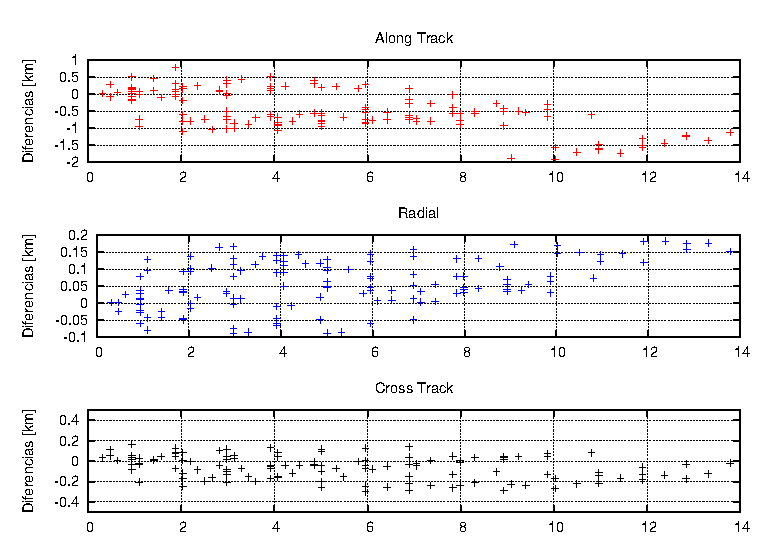
\includegraphics[width=0.7\linewidth]{imagenes/vncmultiplot}
%   \caption{A subfigure}
%   \label{fig:sub2}
% \end{subfigure}
% \caption{A figure with two subfigures}
% \label{fig:test}
% \end{figure}

\section{Transformaci\'on de Coordenadas}

Para la comparaci\'on de las posiciones en coordenadas cartesianas, es necesario llevar ambos vectores a un mismo sistema de referencia.
Los datos que provee CODS se publican en el sistema TOD: True of Date (Verdadero de la \'epoca), mientras que los vectores de estado que genera el propagador SGP4 est\'an calculados en el sistema TEME: True Equator Mean Equinox (Ecuador Verdadero y Equinoccio Medio)

\begin{figure}
  \includegraphics[width=\textwidth]{imagenes/sistReferencias}
\end{figure}



\include{secciones/Disenio}
%\chapter{ARxCODE}
\label{chap:arxcode} 

\section{Especificaciones}
Python y PyQT
Donde corre y con que performance.
....


\section{Diseño y Desarrollo}
En el IDE EClipse
Funciones enteramente documentadas (Doxigen).
Control de Versiones (GitHub) - graficos de los tiempos de desarrollo. ¿?


\subsection{Arquitectura}
{\bf{Interfaces.}}\\
clases principales: TLE, EphemCODS
\subsection{parametros globales y nomenclatura de la generacion de archivos}
Parametros:\\
\begin{itemize}
 \item satId
 \item fechaIni,fechaFin
 \item TLE/CODS
\end{itemize}

l prototipo de software para el An\'alisis de Riesgo por Colisi\'on con Desechos Espaciales {\it{ARxCODE}}, ser\'a un sistema anexo a las estructuras ya existentes dentro del departamento de Din\'amica Orbital.\\
El mismo se piensa como un intermediario capaz de: detectar los mensajes de alerta CDM provistos por el JSpOC, procesar los datos, generar mejores estimaciones para la posici\'on del desecho, solicitar datos m\'as precisos para la posici\'on de la misi\'on primaria y calcular la PoC. Todo esto a fin de facilitarle a un a un operador analista experto, herramientas para la toma de decisiones o el intercambio de informaci\'on con los organismos externos y el centro de control.\\

\begin{figure}
  \includegraphics[width=0.8\textwidth]{imagenes/interfasessistemas}
\end{figure}

\subsection*{Requerimientos Funcionales}
\begin{itemize}
\item El sistema deber\'a funcionar en todo momento.\\
\item El software detectar\'a la llegada de un CDM y ser\'a capaz de desglozarlo para extraer la informaci\'on que sea necesaria.\\
\item El software identificar\'a los objetos y solicitar\'a informaci\'on orbital al departamento de Din\'amica Orbital en el caso de la misi\'on principal, y TLEs, en la p\'agina Space-Track, en el caso del desecho.\\
\item El software ajustar\'a la precisi\'on en la posici\'on del desecho y generar\'a la matriz de varianza-covarianza para el mismo.\\
\item El software calcular\'a la PoC.\\
\item El software generar\'a reportes, notificaciones y visualizaciones para facilitar la comprensi\'on y el an\'alisis del riesgo.
\end{itemize}

\subsubsection*{Funcionalidades:}
\begin{itemize}
\item Detectar la recepi\'on de un nuevo mensaje de alerta.\\
\item Extraer la informaci\'on del mensaje y adaptarla al formato necesario.\\
\item Extraer de la web (via spacetrack) los TLEs del desecho involucrado.\\
\item Identificar la misi\'on primaria y solicitar a DO {\color{red}{los datos orbitales precisos necesarios: posici\'on $+$ error}}\\
\item Propagar y ajustar la posici\'on del desecho al TCA, con su error asosciado\\
\item Construir las Matrices Varcorvar.\\
\item Calcular la PoC.\\ 
\end{itemize}


\label{sec:arqydis}

\chapter{Validaci\'on y Resultados}
\label{chap:resultados}

%\endinput

\section{Introducci\'on}
En este cap\'itulo se presentan los distintos escenarios que fueron planteados para la validaci\'on de los procesos.\\

Dado que para la metodolog\'ia de estimaci\'on de errores que proponemos, utilizamos datos reales de una misi\'on operativa argentina, hubiera sido
deseable contar con datos de alertas de colisiones reales propios de esa misi\'on, ya que esto hubiera permitido hacer una validaci\'on end-to-end de todo el prototipo. No obstante, por cuestiones de confidencialidad, no fue posible tener acceso a esa informaci\'on.
Frente a este panorama, se detalla a continuaci\'on la secuencia de etapas de validaci\'on que permiten evaluar, cada una de las instancias del procesamiento.\\

En primer lugar fue fundamental corroborar las propagaciones de los TLE realizadas con la librer\'ia de python {\it{sgp4-1}} \citep{sgp4python}, para ello utilizamos la versi\'on de prueba que ofrece el software STK: {\it{System Tool Kit}}, \citep{stk}.\\

Para la validaci\'on de los resultados de la implementaci\'on del m\'etodo de Osweiler en la generaci\'on de matrices de covarianza, se compararon los resultados de ARxCODE para dos de los escenarios que se publican en el trabajo.\\

El m\'etodo que se propone para la estimaci\'on de la propagaci\'on de errores, es el que m\'as dificultades present\'o para ser validado. Al basarse plenamente en los datos de la misi\'on cuyos resultados de colisi\'on de alerta no pudieron ser suministrados, fue analizado en comparaci\'on con resultados estad\'isticos globales, o sobre el estudio de encuentros de otras misiones.\\

Finalmente la implementaci\'on del c\'alculo de probabilidad de colisi\'on fue evaluada a partir de registros p\'ublicos de encuentros anteriores recopilados de internet en formato de correos electr\'onicos o CDM; y tomando datos de estudios publicados en el libro de Klinkrad \citep{Klinkrad} y en el trabajo de Xu y Xiong \citep{xu2014method}\\

\section{Implementaci\'on del modelo SGP4 en Python}

Para la propagaci\'on de las posiciones orbitales con el modelo SGP4 (Sec. \ref{subsec:sgp4model}) utilizamos la librer\'ia de python {\bf{sgp4-1}} \citep{sgp4python}.
Luego usamos el software STK para comparar nuestras propagaciones y asegurarnos la correcta utilizaci\'on y configuraci\'on de la librer\'ia sgp4-1.\\

Las Tablas \ref{tab:arcode}  y \ref{tab:stk} muestran las efem\'erides de la misi\'on operativa durante los primeros cuatro minutos del d\'ia 01/01/2013.
Ambas fueron generadas a partir del mismo TLE y presentan resultados que difieren en algunos metros para los peores casos. Resultado aceptable, teniendo en cuenta que las estimaciones groseras de errores para las propagaciones hechas con TLEs y SGP4 acarrean errores de kil\'ometros o decenas de kil\'ometros.\\

\underline{TLE.}
{\small
\begin{verbatim}
1 xxxxU xxxxx   13001.74853505  .00000428  00000-0  75550-4 0  9996
2 xxxxx 098.0122 011.5654 0001526 107.5603 009.0604 14.72289948 84036
\end{verbatim}}


\begin{table}[!h]
\caption{Resultados que genera ARxCODE utilizando la librer\'ia sgp4 de python para la propagaci\'on.}
\centering
\resizebox{17cm}{!}{
\begin{tabular}{lcccccc}
\hline
Epoca & x [km] & y [km] & z [km] & vx $[km/s]$ & vy $[km/s]$ & vz $[km/s]$\\
\hline
2013-01-01 00:00&-2372.76245& -1381.01830& 6465.57494& -6.95099& -0.93631& -2.74523\\
2013-01-01 00:01& -2784.64672& -1434.31269& 6287.6158& -6.77374& -0.83955& -3.18470\\
2013-01-01 00:02& -3185.05363& -1481.69530& 6083.67196& -6.56854& -0.73932& -3.61109\\
2013-01-01 00:03& -3572.3305& -1522.96975& 5854.58154& -6.336229& -0.63602& -4.02263\\
2013-01-01 00:04& -3944.8780& -1557.96472& 5601.28702& -6.077737& -0.53007& -4.417616\\
\hline
\label{tab:arcode}
\end{tabular}
}
\end{table}

\begin{table}[!h]
\caption{Resultados del Systems Tool Kit (STK) propagando el mismo TLE que ARxCODE.}
\centering
\resizebox{17cm}{!}{
\begin{tabular}{lcccccc}
\hline
\'Epoca & x [km] & y [km] & z [km] & vx [km/s] & vy [km/s] & vz [km/s]\\
\hline
2013-01-01 00:00&-2372.76302&-1381.02018&6465.57433&-6.95099&-0.93631&-2.74523\\
2013-01-01 00:01&-2784.64726&-1434.31473&6287.61518&-6.77374&-0.83955&-3.18470\\
2013-01-01 00:02&-3185.05413&-1481.69750&6083.67116&-6.56854&-0.73932&-3.61109\\
2013-01-01 00:03&-3572.33097&-1522.97210&5854.58064&-6.33622&-0.63602&-4.02263\\
2013-01-01 00:04&-3944.87849&-1557.96721&5601.28604&-6.07773&-0.53008&-4.41761\\
\hline
\label{tab:stk}
\end{tabular}
}
\end{table}


%\textcolor{red}{hacer las diferencias medias para todo un dia en python y publicarlas}

\section{Estudio de errores de TLE con datos hist\'oricos}

El trabajo de Osweiler publica los resultados de las matrices de covarianza generadas, para 6 misiones y 8 ventanas de tiempo.
Para la validaci\'on se tomaron dos escenarios muy diferentes en cuanto a la altura del sat\'elite: LAGEOS-1 a m\'as de $5000$ km y ICESAT a $600 $ km, (Tabla \ref{tab:satescenarios}).

\begin{table}[!h]
\caption[Sat\'elites de Estudio]{Resumen de las caracter\'isticas de los sat\'elites a analizar.}

      \begin{tabular}{cccccc}
      \hline
      Nombre & ID NORAD & Altura & Ecc. & Inclinaci\'on & B* \\
      \hline
      LAGEOS-1 & 8820 & $5850$ & $0.004$ & $109.8$ & $0.0001$ \\
      ICESAT & 27642 & $600$ & $0.0002 - 0.001$ & $94$ & var\'ia \\
      \hline
      \end{tabular}
    \label{tab:satescenarios}
\end{table}

Se presentan a continuaci\'on las tablas con los resultados comparativos, entre los valores publicados (Tablas \ref{tab:icesatOSW} y \ref{tab:lageosOSW}) y los valores obtenidos por ARxCODE (Tablas \ref{tab:icesatARX} y \ref{tab:lageosARX}) para una \'unica ventana temporal.\\

Puede apreciarse, que los errores son muy grandes para el ICESAT, de baja altura, que se ve m\'as perturbado por el efecto atmosf\'erico, que no es modelable con precisión; mientras que el LAGEOS-1 presenta errores muchos \'ordenes de magnitud menor.\\

\subsection*{Tablas comparativas ICESAT}

\begin{table}[!h]
\centering
\makebox[0pt][c]{\parbox{1.0\textwidth}{%
    \begin{minipage}[t]{0.48\hsize}
    \caption{Matriz de Covarianza. \citep{osweiler} \\ ICESAT del 1-Mar-03 al 16-Mar-03.}
     \resizebox{8cm}{!}{
    \begin{tabular}{cccc}
      \hline
    Vent 1 & $R_{v}$ (km) & $R_{n}$ (km) & $R_{c}$ (km)\\
    \hline
    $R_{v}$ &  2667.377375  &    27.248658   &   -8.22221222\\
    $R_{n}$ & 27.248658  &   0.34323269 & -0.12314379\\
    $R_{c}$ & -8.22221222 & -0.12314379 & 0.07316443\\
    \hline
    \end{tabular}}
      \label{tab:icesatOSW}
    \end{minipage}
    \begin{minipage}[t]{0.48\hsize}
    \caption{Matriz de Covarianza de ARxCODE. \\ ICESAT del 1-Mar-03 al 16-Mar-03.}
    \resizebox{8cm}{!}{
      \begin{tabular}{cccc}
	\hline
      Vent 1 & $R_{v}$ (km) & $R_{n}$ (km) & $R_{c}$ (km)\\
      \hline
      $R_{v}$ &  2667.37364259 &   27.2488814  &   -8.22232626\\
      $R_{n}$ & 27.2488814  &  0.3432413 &  -0.12314867\\
      $R_{c}$ & -8.22232626 & -0.12314867 &  0.073167\\
      \hline
      \end{tabular}}
        \label{tab:icesatARX}
    \end{minipage}
 %   \hfill
}}
\end{table}

\begin{table}[!h]
\caption{Diferencias de ARxCODE respecto a Osweiler \citep{osweiler}}

  \begin{tabular}{cccc}
  \hline
 Vent 1 & Dif.$R_{v}$ (km) & Dif.$R_{n}$ (km) & Dif.$R_{c}$ (km)\\
 \hline
 Dif. $R_{v}$ & -0.00373241 & 0.0002234 & -0.00011404 \\
 Dif. $R_{n}$ &  0.0002234 &  0.000008 & -0.000004\\
 Dif. $R_{c}$ & -0.00011404  & -0.000004 &  0.000002\\
 \hline
 \end{tabular}
 \label{tab:icesatcomp}
\end{table}


\subsection*{Tablas comparativas LAGEOS-1}

\begin{table}
\centering
\makebox[0pt][c]{\parbox{1.0\textwidth}{%
    \begin{minipage}[b]{0.48\hsize}
    \caption{Matriz de Covarianza. \citep{osweiler} \\ LAGEOS-1 del 1-Mar-03 al 16-Mar-03}
    \resizebox{8cm}{!}{
      \begin{tabular}{cccc}
	\hline
      Vent 1 & $R_{v}$ (km) & $R_{n}$ (km) & $R_{c}$ (km)\\
      \hline
      $R_{v}$ &  0.37863904 & -0.03440871 & 0.02772177 \\
      $R_{n}$ & -0.03440871 & 0.00401173 & -0.00272334 \\
      $R_{c}$ & 0.02772177 & -0.00272334 & 0.00843443\\
      \hline
      \end{tabular}}
        \label{tab:lageosOSW}
    \end{minipage}
    \hfill
    \begin{minipage}[b]{0.48\hsize}
    \caption{Matriz de Covarianza de ARxCODE \\ LAGEOS-1 del 1-Mar-03 al 16-Mar-03}
     \resizebox{7.5cm}{!}{
    \begin{tabular}{cccc}
      \hline
    Vent 1 & $R_{v}$ (km) & $R_{n}$ (km) & $R_{c}$ (km)\\
    \hline
    $R_{v}$ & 0.378619 & -0.0343598 & 0.02771527 \\
    $R_{n}$ & -0.0343598 &  0.004002 & -0.0027171 \\
    $R_{c}$ & 0.02771527 & -0.0027171 &  0.0084302 \\
    \hline
    \end{tabular}}
      \label{tab:lageosARX}
   \end{minipage}
    \hfill
}}
\end{table}

\begin{table}
\caption{Diferencias de ARxCODE respecto a Osweiler, \citep{osweiler}.}
 \begin{tabular}{cccc}
  \hline
 Vent 1 & Dif.$R_{v}$ (km) & Dif.$R_{n}$ (km) & Dif.$R_{c}$ (km)\\
 \hline
 Dif. $R_{v}$ & 0.000020 &  -0.000048 &  0.000006 \\
 Dif. $R_{n}$ & -0.000048 &   0.000009 &  -0.000006 \\
 Dif. $R_{c}$ & 0.000006 &  -0.000006 &   0.000004 \\
 \hline
 \end{tabular}
 \label{tab:lageoscomp}
\end{table}

Las diferencias que resultan en la comparaci\'on con los resultados que arroja ARxCODE, son todas menores a los metros (Tablas \ref{tab:icesatcomp} y \ref{tab:lageoscomp}). En particular LAGEOS muestra errores menores que ICESAT, ya que al ser un sat\'elite a mayor altura, el efecto atmosf\'erico es menor y el modelo de propagaci\'on, se adapta mejor.\\

\subsection*{Diferencias de los escenarios iterando el TLE primario en el m\'etodo de Osweiler}
Estudio hecho sobre los errores que se producen en las propagaciones de los TLE en funci\'on de la cantidad de d\'ias que se propaguen.
Estos resultados ofrecen mayor informaci\'on respecto a los errores que se cometen en funci\'on de la cantidad de d\'ias que se propagan los TLE.\\

Para la generaci\'on de los datos, se propagaron todos los TLE del conjunto hacia las fechas de todos los TLE con fechas m\'as actualizadas, dentro del conjunto (Fig. \ref{fig:todosOSW}). Las diferencias que resultaron se plasman en funci\'on del intervalo de propagaci\'on, en las Figuras \ref{fig:icesatTot} y \ref{fig:lageosTot} para el ICESAT y el LAGEOS respectivamente. 

\begin{figure}[!h]
\centering
  \textbf{Propagaci\'on y comparaci\'on de TLE }\par\medskip
  \fbox{\includegraphics[width=0.8\textwidth]{imagenes/todosOSW}}
  \caption{Esquematizaci\'on del algoritmo para comparar la propagaci\'on de cada TLE del set hacia fechas futuras de los TLE del set. Extra\'ido del trabajo de Osweiler, \citep{osweiler}}.
  \label{fig:todosOSW}
\end{figure}

\begin{figure}[h!]
\centering
  \subfigure[Diferencias ICESAT - ARxCODE]{
    \includegraphics[width=0.48\textwidth]{imagenes/TLEdifTot27642esc52}
  }
  \subfigure[Diferencias ICESAT - Osweiler, \citep{osweiler}]{
    \includegraphics[width=0.48\columnwidth, keepaspectratio]{imagenes/ICESATdifTot}
  }
  \caption{Gr\'afico con Diferencias Totales del escenario ICESAT}
  \label{fig:icesatTot}
\end{figure}

\begin{figure}[h!]
\centering
  \subfigure[Diferencias LAGEOS-1 - ARxCODE]{
    \includegraphics[width=0.48\textwidth]{imagenes/TLEdifTot8820esc11}
  }
  \subfigure[Diferencias LAGEOS-1 - Osweiler, \citep{osweiler}]{
    \includegraphics[width=0.48\columnwidth, keepaspectratio]{imagenes/LAGEOSdifTot}
  }
  \caption{Gr\'afico con Diferencias Totales del escenario LAGEOS-1}
  \label{fig:lageosTot}
\end{figure}

Los errores que se observan en la propagaci\'on de TLE, en funci\'on de la cantidad de d\'ias propagados, muestran comportamientos casi id\'enticos.\\

En este estudio, puede apreciarse una clara diferencia en las cotas de los errores, siendo el sat\'elite ICESAT, de menor altura el que muestra errores mayores en un rango de -120 a 60 km, mientras que el LAGEOS, contiene las diferencias entre -2 y 1 km.\\

No obstante, en ambos se distingue, que la componente asociada a la velocidad (V {\it{in-track}}) es la que mayor error acumula en propagaciones m\'as largas. Esto se debe a que el modelo es d\'ebil en cuanto a la perturbaci\'on que introduce la atm\'osfera, directamente vinculada a la velocidad de los objetos para el caso del ICESAT o en cuanto al modelo que describe la presi\'on de radiaci\'on solar en el caso del LAGEOS.\\

Se concluye a partir de esta secci\'on, que ARxCODE implementa el m\'etodo de Osweiler y la construcci\'on de las diferencias de pares correctamente. 

\section{Estudio de errores de TLE con efem\'erides precisas}
\subsection*{Sistema de referencia TOD}
La misi\'on operativa ofrece mediciones propias de sus efem\'erides. En esta secci\'on se muestran los resultados de comparar las posiciones obtenidas mediante los datos p\'ublicos TLE, propagadas con SGP4, contra las efem\'erides precisas.\\ 

En primer lugar fue necesario plasmar las posiciones en el mismo sistema de referencia, ya que los productos del departamento de din\'amica orbital con los que trabajamos ofrecen las posiciones orbitales en el sistema de referencia verdadero de la fecha \ac{TOD}, mientras que los resultados de las propagaciones con el SGP4 se encuentran en el sistema \ac{TEME}. Para poder hacer comparaciones desarrollamos un m\'odulo que transforma las coordenadas y velocidades, del sistema TEME al sistema TOD (Ap\'endice. \ref{App1}).\\

Para la validaci\'on del mismo, utilizamos TLE de la misi\'on y los propagamos con el SGP4. Los resultados que obtuvimos (en el sistema TEME), los transformamos al sistema TOD con el m\'odulo de transformaci\'on desarrollado y luego lo comparamos con los productos del STK, corridos para el mismo TLE y publicados en el sistema TOD que STK ofrece. Las comparaciones se hicieron para propagaciones con paso de 1 minuto a lo largo de todo el dia 01 de Enero de 2013. Los resultados mostraron diferencias menores a los mil\'imetros, de manera que el algoritmo puede usarse sin que incorpore errores significativos  (Tabla \ref{tab:compprecisas}).\\

\begin{table}[!h]
\caption{Comparaci\'on entre ARxCODE y STK de \\la transformaci\'on de TEME a TOD.}
\begin{tabular}{l|c}
  \hline
  Coordenada  X &  0.0003168 [m]\\
  Coordenada Y &  0.0006370 [m]\\
  Coordenada Z &  0.0005133 [m]\\
  \hline
\end{tabular}
\label{tab:compprecisas}
\begin{flushleft}
\small 1 de Enero de 2013, paso 1 minuto.
\end{flushleft}

\end{table}

\subsection*{Estad\'istica de Errores}
Con la certeza de que los datos eran compatibles y pod\'ian ser comparados (ambos se referencian en el sistema TOD), se inici\'o el procesamiento de comparaci\'on de las posiciones de las efem\'erides precisas de la misi\'on y las propagaciones de los TLE, para la estimaci\'on de los errores de la propagaci\'on, (Sec. \ref{subsec:errorProp}).\\

En un pre-procesamiento sobre un periodo amplio de la misi\'on, constatamos que fuera de los intervalos de maniobras por {\it{commissioning}}\footnote{Puesta en \'orbita nominal} o maniobras de rutina, los TLE presentan un error que es {\it{acotado}}, {\it{estable}} y/o modelable. \\

Las comparaciones de las propagaciones de los TLE mostraron significativas aleatoriedades y amplias diferencias en el estudio realizado con los datos correspondientes al a\~no 2012, no obstante los resultados del estudio con datos del a\~no 2013 mostraron la tendencia y estabilidad esperada, con errores m\'aximos del orden de las decenas de kil\'ometros (Fig. \ref{fig:sacd2013}).


\begin{figure}[!h]
\centering
  \textbf{Tendencia Anual 01/01/2013 - 30/08/2013}\par\medskip
  \includegraphics[width=\textwidth]{imagenes/SACD2013todEjesajustados}
  \caption{Tendencia anual de las diferencias contra los datos de din\'amica orbital en coordenadas cartesianas del Sistema TOD}
  \label{fig:sacd2013}
\end{figure}

\subsection*{Generaci\'on de la tabla de propagaci\'on de errores}

Como se explic\'o en la Sec. \ref{subsec:errorProp}, para estimar los errores en la propagaci\'on se propone un m\'etodo que utiliza una tabla (Tabla \ref{tab:resultatabla}), generada a partir de la estad\'istica que resulta de comparar las propagaciones de los TLE de la misi\'on operativa, con las efem\'erides precisas. Las comparaciones se hacen en el periodo de Enero a Junio del a\~no 2013, en intervalos de 1 a 6 d\'ias, con paso 1 segundo.\\

\begin{table}[!h]
\caption[Tabla con los valores medios para la propagaci\'on de errores.]{Valores medios de las varianzas calculadas para la propagaci\'on de errores.\\ Autor\'ia propia.}
\begin{tabular}{lccc}
\hline \hline
\rowcolor{yellow!35}
&$\sigma^{2}_R [km]$ &$\sigma^{2}_T [km]$ &$\sigma^{2}_N [km]$\\
\hline \hline
< 1 d\'ia & 0.05287535953&0.5110606907&0.09802202353\\
\hline
1 d\'ia & 0.03846388969&0.4517572281&0.09807457894\\
\hline
2 d\'ias & 0.02760890529&0.4086434248&0.09904162392\\
\hline
3 d\'ias & 0.01963580775&0.3765098311&0.09022336881\\
\hline
4 d\'ias & 0.01469071678&0.3577884914&0.1182060362\\
\hline
5 d\'ias & 0.01332578794&0.3557767231&0.1264764812\\
\hline
6 d\'ias & 0.01524829841&0.365815954&0.1607439516\\
\hline
\end{tabular}
\label{tab:resultatabla}
\end{table}

Los resultados que se encuentran, no es posible validarlos directamente. No obstante, son comparables a los que proponen Flohrer et al., \citep{flohrer2008assessment}, en la {\it{lookup table}} generada considerando todos los objetos del cat\'alogo al 01 de Enero de 2008 (Fig.  \ref{fig:flohrer}). Los valores de las desviaciones est\'andar que resultan del m\'etodo propuesto son menores casi en un orden de magnitud a las tablas gen\'ericas que publican Flohrer et al., \citep{flohrer2008assessment}, esto es de esperar, ya que los estudios de la publicaci\'on son m\'as abarcativos y gen\'ericos.\\

\begin{figure}[!h]
  \centering
  \fbox{\includegraphics[width=0.6\textwidth]{imagenes/flohrertabla}}
  \caption{{\it{Look-up table}} [metros] de los resultados promediados del an\'alisis del cat\'ologo completo al 01 de Enero de 2008, de los errores en las coordenadas UVW, clasificados por excentricidad, inclinaci\'on y altura. Se resaltan en celeste las celdas correspondientes a la configuraci\'on de la misi\'on operativa que se utiliz\'o en este trabajo. Extra\'ido de Flohrer et al., \citep{flohrer2008assessment}}.
  \label{fig:flohrer}
\end{figure}

% \begin{itemize}
%  \item Klinkrad Tabla para 14 misiones.
%  \item Paper del research gate
%  \item Peterson?!
% \end{itemize}
% 
% FINALIZAR CON COMPARACI\'ON TLE vs TLE. 

\section{C\'alculo de la Probabilidad de Colisi\'on}

Hasta este punto, se han validado cada uno de los procesos por separado.
Resta hacer pruebas desde el origen, es decir a partir de identificar los objetos y el TCA, correr los procesamientos de ARxCODE y obtener los resultados de la PoC.
A tal fin, fue necesario conseguir registros que contuvieran la informaci\'on completa de una situaci\'on de encuentro.\\

\subsection*{Casos de Prueba}
Por un lado se consiguieron correos electr\'onicos de alerta p\'ublicos en internet, y por otro CDMs tambi\'en p\'ublicos\footnote{https://cwe.ccsds.org/moims/docs/Forms/AllItems.aspx?RootFolder=\%2Fmoims\%2Fdocs\%2FMOIMS-NAV\%2FDraft\%20Documents\%2FConjunction\%20Data\%20Message\%20\%28CDM\%29}, pero ninguno de esos datos se corresponden con la misi\'on operativa, cuyas efem\'erides precisas analizamos y utilizamos en la construcci\'on del modelo estad\'istico de propagaci\'on de errores.
As\'i mismo, ni los correos encontrados ni los CDM descargados contienen informaci\'on de la PoC asociada al encuentro. 

Formato de los correos electr\'onicos:
\begin{center}
\fbox{\parbox[b]{0.8\linewidth}{\small{
The United States Joint Space Operations Center (JSpOC) has identified a\\
predicted conjunction between DELFI C3 (SCC\# 32789) and SCC\# 23657.\\

Primary Object: DELFI C3 (SCC\# 32789)\\
Secondary Object: SCC\# 23657\\
Time of Closest Approach: 15 JUL 2012 21:21 UTC \\

Overall miss distance: 760 meters\\
Radial (dU) miss distance: -186 meters\\
In-Track (dV) miss distance: -389 meters\\
Cross-track (dW) miss distance: -626 meters\\

Primary Radial Error (U): 38 meters\\
Primary In-track Error (V): 1388 meters\\
Primary Cross-track Error (W): 11 meters\\

Secondary Radial Error (U): 8 meters\\
Secondary In-track Error (V): 338 meters\\
Secondary Cross-track Error (W): 2 meters\\}
}}\label{box:mail}
\end{center}


La Figura \ref{fig:tablamails}, muestra el resumen de la informaci\'on de todos los correos electr\'onicos fueron procesados con ARxCODE. 
\begin{figure}[!h]
  \centering
  \fbox{\includegraphics[width=\textwidth]{imagenes/tablamails}}
  \caption{Contenido de los correos electr\'onicos utilizados para comparar los resultados.}
  \label{fig:tablamails}
\end{figure}

Se listan a continuaci\'on los seis CDM cuyos datos fueron procesados con ARxCODE (Fig. \ref{fig:cdmsproc}). 

 \begin{figure}[!h]
  \centering
  \fbox{\includegraphics[width=\textwidth]{imagenes/tablaCDM}}
  \caption{Contenido de los CDM utilizados para comparar los resultados.}
  \label{fig:cdmsproc}
\end{figure}

Por \'ultimo se analizaron diez casos de prueba: cuatro casos publicados mediante el servicio web de SOCRATES \citep{Kelso} que ofrece Celestrack,  dos casos  presentados en el libro de Klinkrad \citep{KlinkradChapter8} y cuatro casos publicados por Xu-Xiong \citep{xu2014method}, que contienen los datos iniciales necesarios para disparar el procesamiento y los valores de la PoC.\\

DECIR ALGO DE SOCRATES.
\begin{table}[!h]
 \caption{Casos de Prueba tomados del servicio SOCRATES \citep{Kelso}.}
\resizebox{13cm}{!}{
\begin{tabular}{lccccccc}
 \hline \hline
  \rowcolor{lightgray}
 \# & sat id & deb id & TCA & Min Dist [km] & PoC  \\
 \hline
 1 & 41456 & 35732 & 29-06-2018 22:22:48.14 & 0.039 & 1.74e-03 \\
 2 & 33412 & 19008 & 30-06-2018 03:42:30.937 & 0.096 & 2.62e-04\\
 3 & 27386 & 35519 & 25-05-2018 09:46:17.533 & 0.926 & 1.10e-04\\
 4 & 27386 & 37887 & 08-07-2018 23:36:38.326 & 0.137 & 6.10e-04\\
 \hline
\end{tabular} }
\label{tab:escenariosSOCRATES}
\end{table}

En el cap\'itulo ocho de su libro, Klinkrad \citep{Klinkrad}, publica una tabla que contiene siete situaciones de encuentros de riesgo para las misiones ENVISAT y ERS-2. De esos escenarios s\'olo se han podido reproducir dos, ya que no fue posible identificar los c\'odigos de NORAD de los desechos involucrados en el resto de los encuentros.

\begin{table}[!h]
 \caption{Casos de prueba tomados del libro de Klinkrad \citep{Klinkrad}.}
\resizebox{13cm}{!}{
\begin{tabular}{lccccccc}
 \hline \hline
  \rowcolor{lightgray}
\# & sat id & deb id & TCA & Min Dist [km] & PoC  \\
 \hline
 5 & 27386 &  12442 & 2004-09-02 19:14:11 & 1.297& 2.186e-04\\
 6 & 23560 &  16681 & 2004-09-29 23:56:02 & 0.067& 1.546e-04\\
 \hline
\end{tabular} }
\label{tab:escenariosKlinkrad}
\end{table}

En un mismo sentido, se utilizaron los valores publicados en el trabajo de Xu y  Xiong, \citep{xu2014method}, donde  se presentan las estimaciones de la m\'inima distancia y la Poc, utilizando un m\'etodo general y el m\'etodo desarrollados por ellos (Tabla \ref{tab:escenariosxx}).\\

\begin{table}[!h]
\caption{Casos de prueba tomados del trabajo de  Xu \& Xiong \citep{xu2014method}.}
\resizebox{15cm}{!}{
\begin{tabular}{lcccccccc}
 \hline \hline
  \rowcolor{lightgray}
\# & sat id & deb id & TCA & Min Dist [km] & PoC (general) & PoC \\
 \hline
 7  & 25415 & 31445 & 2013-03-18 14:44:34 & 0.115 & 1.24e-05  & 1.52e-05\\
 8  & 20737 & 20738 & 2013-03-17 10:39:31 & 0.104 & 1.706e-06 & 2.15e-06\\
 9  & 27939 & 31588 & 2013-03-16 13:46:21 & 0.098 & 3.01e-05  & 3.51e-05 \\
 10 & 11308 & 32315 & 2013-03-15 03:02:16 & 0.094 & 1.8e-05   & 2.05e-05\\
 \hline
\end{tabular} }
\label{tab:escenariosxx}
\end{table}

\subsection*{Implementaci\'on de los algoritmos de c\'alculo de PoC}
En este trabajo se utilizaron tres m\'etodos distintos para estimar el valor de la PoC. El primero de ellos, que denominamos {\it{m\'etodo del l\'imite}}, es una simple expresi\'on que resulta como conclusi\'on de un trabajo de Alfano \citep{Alfano}, y dado que resulta una implementaci\'on muy sencilla no realizamos ninguna prueba para evaluarla.

El segundo de los m\'etodos es el que propone Lei-Chen \citep{leichen}. Tambi\'en consiste en una simple expresi\'on pero el resultado puede compararse con la resoluci\'on de la integral num\'erica que el m\'etodo aproxima. A su vez las variables que se introducen en la ecuaci\'on deben ser previamente transformadas al sistema de referencia RSW. En este caso fue posible aprovechar un ejemplo que el propio Lei-Chen incorpora en su libro para verificar la correcta implementaci\'on del algoritmo.  

\subsubsection*{Comparaci\'on de los resultados con la resoluci\'on de la integral}
Se toman como datos iniciales, los valores publicados por el propio autor Lei-Chen, \citep{leichen}, y se calcula la PoC, tanto para la expresi\'on anal\'itica como la integral. Para esta \'ultima se utiliza la biblioteca {\it{scipy.integrate}}  de python.\\

De las expresiones para el c\'alculo de la PoC (Eq. \ref{eq:pocintegral} y Eq. \ref{eq:pocexpress}), se desprende que ser\'an necesarios los datos: ($\mu_{x}, \mu_{y}$), ($\sigma_{x}, \sigma_{y}$), $r_{a}$.\\

Se tomaron los datos que utiliza Lei-Chen en el ejemplo para el caso de las \'orbitas circulares y se calcul\'o la PoC a partir de la expresi\'on expl\'icita y realizando la integral.\\

\begin{minipage}[t]{0.28\textwidth}
{\bf{Valores iniciales.}}\\

\begin{tabular}{|lc|}
\hline
 Dato & valor \\
\hline
$\mu_{x}$ & 0.031731 [km]\\
$\mu_{y}$ & 0.697294 [km]\\
$\sigma_{x}$ & 0.0430576\\
$\sigma_{y}$ & 0.2941297\\
$r_{a}$ & 0.01 [km]\\
\hline
\end{tabular}
\end{minipage}
\begin{minipage}[t]{0.7\textwidth}
\begin{mdframed}[
        linecolor=red,linewidth=2pt,% 
        frametitlerule=true,% 
        apptotikzsetting={\tikzset{mdfframetitlebackground/.append style={%
            shade,left color=white, right color=blue!20}}}, 
        frametitlerulecolor=blue,
        frametitlerulewidth=1pt, innertopmargin=\topskip,
        frametitle={Probabilidad de Colisi\'on},
        outerlinewidth=1.25pt
    ]
\large
\captionof{table}{Resultados Comparativos del c\'alculo de la PoC.}
\begin{tabular}{|l|l|l|}
  \hline
 Te\'orico & Expresi\'on & Valor de la Integral\\
 \hline
 1.8079750e-04 & 1.8079124e-04 & 1.8071110e-04\\
 \hline
\end{tabular}
\label{tab:poccomp}
\end{mdframed}
\end{minipage}

\vspace{0.5cm}
Como se observa en el recuadro de las probabilidades de colisi\'on (Tabla \ref{tab:poccomp}); las f\'ormulas implementadas coinciden con el valor de la bibliograf\'ia hasta el cuarto d\'igito significativo de la expresi\'on.\\

En este punto se confirma que, una vez que se obtiene: $\mu_{x}$, $\mu_{x}$, $\sigma_{x}$, $\sigma_{y}$ y el radio de colisi\'on $r_{a}$, ya puede calcularse la PoC. 
Ahora resta verificar, paso a paso c\'omo llegar de los inputs de ARxCODE, a estos par\'ametros que se introducen en de las ecuaciones. \\

\subsubsection*{Transformaci\'on al sistema de referencia RSW}

Una vez determinadas la posici\'on relativa de los objetos en el sistema RSW o RTN en el TCA, la proyecci\'on al plano para \'orbitas circulares, no representa mayores problemas, como se detall\'o en la Sec. \ref{subsec:pocsimp}.\\

Pero es importante verificar, que a partir de las posiciones inerciales de los objetos en el TCA, las transformaciones de la distancia relativa de los mismos al sistema RSW, coinciden.
Para ello, vamos a utilizar las posiciones de los objetos del ejemplo de la bibliograf\'ia (Tabla \ref{tab:vectejemplo}) y transformarlas con el m\'odulo de transformaci\'on {\it{sisRic}} del paquete {\it{SistReferencia.SistdeCoordenadas}} para corroborar los resultados.
\\

\begin{table}[!h]
\caption{Vectores de Posiciones Inerciales al momento TCA.}
\begin{tabular}{lcccccc}
\hline
Objeto & x [km] & y [km] &z[km] &vx [km/s] &vy [km/s] &vz [km/s]\\
\hline
Obj1 & 1457.273246 &1589.568484&6814.189959&7.001731&2.439512&0.926209\\
Obj2 & 1457.532155&1588.932671&6814.316188&3.578705&6.172896&2.200215\\
\hline
\end{tabular}
\label{tab:vectejemplo}
\begin{flushleft}
\small {\it{Nota.}} Extra\'idos del ejemplo de la bibliograf\'ia \citep{leichen}.
\end{flushleft}
\end{table}

\begin{table}[!h]
\caption{Comparaci\'on entre el m\'odulo {\it{sisRic}} de autor\'ia propia \\y los datos de Lei-Chen \citep{leichen}.}
\begin{tabular}{lccc}
\hline
Resultados seg\'un & R [km] & S [km] & W[km] \\
\hline
Lei Chen & 0.031731& 0.436476&0.543785\\
ARxCODE & 0.031797& 0.462295 &0.522013
\\
\hline
\end{tabular}
\label{tab:rswcomp}
\end{table}

Estos resultados que se publican en la Tabla \ref{tab:rswcomp}, se logran en una transformaci\'on en la que se considere al Obj2 como origen de la referencia. Los mismos muestran una coincidencia del orden de las decenas de metros, aceptable para estas estimaciones.
No obstante, contando s\'olo con la informaci\'on de los vectores de posici\'on al momento del m\'aximo acercamiento, no es posible verificar el m\'etodo de Osweiler de la construcci\'on de la matriz de covarianza para este ejemplo de la bibliograf\'ia.\\

El \'ultimo de los m\'etodos, el {\it{m\'etodo de Akella \& Alfriend}}, es el m\'as complejo en cuanto a los procedimientos que hay que realizar para hacer el c\'alculo final de la PoC. No obstante no se cuenta con bibliograf\'ia espec\'ifica que contenga valores de la PoC calculados utilizando este m\'etodo. De manera que el mismo ser\'a verificado comparando los resultados con los de los otros m\'etodos.

\subsection*{An\'alisis de los resultados}

\subsubsection*{Validaci\'on con correos electr\'onicos de alerta p\'ublicos}

El proceso de validaci\'on utilizando los correos electr\'onicos obtenidos en la web, consiste en extraer de los correos los identificadores de NORAD de ambos objetos y el TCA asociado al encuentro. A partir de all\'i se calcula la m\'inima distancia total, o sea el m\'odulo de la misma, y  en componentes en el sistema RTN y finalmente la PoC.
Dado que el TCA que se publica en los correos no tiene informaci\'on de los segundos, se realiza una primera estimaci\'on, y luego se profundiza en an\'alisis de la situaci\'on.\\

A partir de esa informaci\'on se carg\'o manualmente el identificador de NORAD del sat\'elite (sat\_id), el identificador de NORAD del desecho (deb\_id), y el TCA de cada situaci\'on; en un primer paso se utiliz\'o ARxCODE para obtener el valor de los segundos del TCA. Luego se propag\'o para el TCA que inclu\'ia los segundos, con pasos de propagaci\'on distintos, en un caso cada un segundo (Tabla \ref{tab:mails1seg}) y en otro caso para un paso menor, de cien mil microsegundos (Tabla \ref{tab:mails100mseg}).\\

\begin{table}[!h]
\caption{ARxCODE a partir de correos electr\'onicos\\ Propagaciones cada 1 segundo - (Radio de colisi\'on $r_{a}=0.01$ km)}
\resizebox{17cm}{!}{
\begin{tabular}{ccrrrrr}
 \hline \hline
 \# & TCA arx & $\Delta R_{arx}$ [km] & $\Delta T_{arx}$ [km] & $\Delta N_{arx}$ [km] & Min Dist. arx [km] & PoC arx\\
 \hline \hline
 1 & 2012-07-15 21:21:51 & 0.147 & 2.749 &  2.287 & 3.579 & 4e-06 \\
 
 2 & 2014-06-29 04:55:59 & 0.081 & 3.921 & 2.002 & 4.403 & 0.0 \\
 
 3 & 2012-11-23 23:38:42 & 0.300 & 1.668 & 0.841 & 1.892 & 0.0 \\

 4 & 2013-03-31 03:25:45 & 68.07& 1.318 & 426.1 & 431.5 & 0.0 \\

 5 & 2013-05-02 17:12:04 & 19.07 & 489.6 & 142.7 & 510.3& 0.0 \\
 \hline
\end{tabular} }
\label{tab:mails1seg}
\end{table}


\begin{table}[!h]
\caption{ARxCODE a partir de correos electr\'onicos\\ Propagaciones cada 100.000 microsegundos - (Radio de colisi\'on $r_{a}=0.01$ km)}
\resizebox{17cm}{!}{
\begin{tabular}{ccrrrrr}
 \hline \hline
 \# & TCA arx & $\Delta R_{arx}$ [km] & $\Delta T_{arx}$ [km] & $\Delta N_{arx}$ [km] & Min Dist. arx [km] & PoC arx\\
 \hline \hline
 1 & 2012-07-15 21:21:51.3 & 0.142 & 0.512 &  0.254 & 0.589 & 4e-06 \\
 
 2 & 2014-06-29 04:55:59.1 & 0.082 & 3.253 & 2.745 & 4.258 & 0.0 \\
 
 3 & 2012-11-23 23:38:42.1 & 0.258 & 0.936 & 1.595 & 1.867 & 1.7e-05 \\
 
 4 & 2013-03-31 03:25:45.1 & 68.07 & 0.194 & 426.1 & 431.5 & 0.0 \\
 
 5 & 2013-05-02 17:12:02.9 & 20.17 & 504.1 & 146.8 & 525.4 & 0.0\\
 \hline
\end{tabular} }
\label{tab:mails100mseg}
\end{table}

\begin{table}[!h]
\caption{M\'inimas distancias de acercamiento para distintos pasos de propagaci\'on y\\ resultados de los los correos electr\'onicos.}
%\resizebox{8cm}{!}{
\begin{tabular}{cccc}
 \hline \hline
  \rowcolor{lightgray}
 \# & Dist (1 seg) [km] & Dist (100 mil $\mu$ seg) [km] & Dist. correo\\
 \hline \hline
 1 & 3.579 &  0.589 &  0.760  \\
 
 2 & 4.403 & 4.258 & 0.334  \\
 
 3 & 1.892 & 1.867 & 0.984 \\
 
 4 & 431.5 & 431.5 & 0.789 \\
 
 5 & 510.3 & 525.4 & 0.170 \\
 \hline
\end{tabular} %}

\label{tab:mailsMinD}
\end{table}

Como puede apreciarse en la Tabla \ref{tab:mailsMinD} de las comparaciones, los distintos pasos de propagaci\'on no modifican los resultados significativamente, salvo en el primer caso. De manera que resulta importante revisar instancias previas, es decir analizar las matrices de error de cada objeto generadas por ARxCODE (Fig. \ref{fig:tablaMAmails}).\\

 \begin{figure}[!h]
  \centering
  \fbox{\includegraphics[width=\textwidth]{imagenes/tablaMAmails}}
  \caption{Tabla con las matrices de covarianza calculadas por ARxCODE (m\'etodo de Osweiler) para la misi\'on y el desecho. Se resaltan los valores que con errores grandes}
  \label{fig:tablaMAmails}
\end{figure}

Se observa, que las matrices calculadas para introducir en el c\'alculo del encuentro de ARxCODE, introducen errores muy grandes y los elementos de su diagonal, correspondientes a las varianzas en cada una de las componentes RTN, son mucho mayores a las que se indican en los mails.\\

De estos resultados se desprende que los valores publicados en los mails, son m\'as precisos a los que se pueden lograr con ARxCODE y seguramente han sido calculados con datos observacionales de rastreo m\'as precisos que la informaci\'on orbital que ofrecen los TLE. 

\subsubsection*{Validaci\'on con CDM p\'ublicos}

A partir de la informaci\'on de los seis CDM, se carg\'o manualmente el identificador de NORAD del sat\'elite (sat\_id), el identificador de NORAD del desecho (deb\_id), el TCA de cada situaci\'on. Se calcul\'o la m\'inima distancia y la PoC, con pasos de propagaci\'on distintos, en un caso cada un segundo (Tabla \ref{tab:cdmsproc1seg}) y en otro caso para un paso menor, de cien mil microsegundos (Tabla \ref{tab:cdmsproc100mseg}).\\
 
 \begin{table}[!h]
  \caption{ARxCODE a partir de los CDM \\ Propagaciones cada 1 segundo - (Radio de colisi\'on $r_{a}=0.01$ km)}
 \centering
 \resizebox{17cm}{!}{
\begin{tabular}{ccrrrrr}
 \hline \hline
 \# & TCA arx & $\Delta R_{arx}$ [km] & $\Delta T_{arx}$ [km] & $\Delta N_{arx}$ [km] & Min Dist. arx [km] & PoC arx\\
 \hline \hline
 1 & 2013-01-10 09:59:57 &0.295626&1.358542&1.321294&1.918033& 1.4e-05 / 1.4e-05\\
 
 2 & 2013-01-12 00:20:51 &0.405629&4.127385&1.632732&4.457091&0.0 / 0.0\\
 
 3 & 2013-01-10 13:22:45 & 0.382972 & 1.173174  & 1.316177 & 1.804252 & 8e-06\\

 4 & 2013-01-11 05:30:56 & 0.01038& 1.276203& 0.648991&1.431779&0.0\\
 
 5 & 2012-11-22 13:03:45.0 & 0.027395 & 4.661372 & 0.332569 & 4.673301 & 1.4e-05/1.4e-05 \\
 
 6 & 2012-12-26 05:00:41 & 0.183897& 4.661359&0.02668&4.665061& 0.0 / 0.0\\
 \hline
 \end{tabular} }

 \label{tab:cdmsproc1seg}
 \end{table}
 
\begin{table}[!h]
 \caption{ARxCODE a partir de los CDM \\ Propagaciones cada 100.000 microsegundos - (Radio de colisi\'on $r_{a}=0.01$ km)}
\centering
 \resizebox{17cm}{!}{
\begin{tabular}{ccrrrrr}
 \hline \hline
 \# & TCA arx & $\Delta R_{arx}$ [km] & $\Delta T_{arx}$ [km] & $\Delta N_{arx}$ [km] & Min Dist. arx [km] & PoC arx\\
 \hline \hline
 1 &2013-01-10 09:59:57  &0.295626&1.358542& 1.321294&1.918033&1.4e-05 \\
 
 2 & 2013-01-12 00:20:51.3 &0.401158&0.140306&0.218037&0.477654&6.1e-05\\
 
 3 & 2013-01-10 13:22:45.2 & 0.382381 &0.288759& 0.043842&0.481165&9e-06\\
 
 4 &2013-01-11 05:30:55.9&0.016754 &0.215364 &0.573953&0.613257&0.0\\
 
 5 & 2012-11-22 13:03:44.7 & 0.023908 & 0.436662& 0.758981 & 0.875955 & 2e-05 \\
 
 6 & 2012-12-26 05:00:40.7 & 0.183162& 0.1859&0.417861&0.492661& 1.24e-04\\
 \hline
 \end{tabular} }
 \label{tab:cdmsproc100mseg}
 \end{table}

 \begin{table}[!h]
 \caption{M\'inimas distancias de acercamiento para distintos pasos de propagaci\'on \\ y resultados de los CDM. (Radio de colisi\'on $r_{a}=0.01$ km)}
\label{tab:cdmsMinD}
\begin{tabular}{lccc}
 \hline \hline
  \rowcolor{lightgray}
 \# & Dist (1 seg) [km] & Dist (100 mil $\mu$ seg) [km] & Dist. CDM\\
 \hline \hline
 1 & 1.918 &  1.918&  0.170 \\
 
 2 & 4.457 & 0.477 & 0.175  \\

 3 & 1.804 & 0.481 & 0.180\\
 
 4 & 1.431 & 0.613 & 0.150\\
 
 5 & 4.665 & 0.875 & 0.976 \\
 
 6 & 4.665 & 0.492 & 0.617\\
 \hline
\end{tabular} 
\end{table}

Para estos \'ultimos procesamientos es notoria la diferencia que se produce cuando se incrementa el paso de propagaci\'on al orden de los cien mil microsegundos; logrando as\'i que los valores calculados por ARxCODE para las m\'inimas distancias se aproximen al valor que publican los CDM.\\

No se pudo identificar a qu\'e se debe esta distinci\'on entre las mejoras que se logran en los CDM, que no se logran en la informaci\'on que proviene de los correos electr\'onicos, aunque probablemente se deba a la incerteza en el TCA que introducen los correos al no informar el TCA con precisi\'on del segundo.\\

\subsubsection*{Validaci\'on con escenarios que incluyen el valor de PoC}

A continuaci\'on se presentan los resultados obtenidos, al procesar cada uno de los diez escenarios  con los tres m\'etodos diferentes.\\ 

Dado que el c\'alculo de la distancia se realiza en primera instancia y es independiente del m\'etodo de c\'omputo de la PoC que se utilice, en la primera Tabla \ref{tab:distlimite} se muestran las diferencias de las distancias calculadas con las publicadas y los valores de las PoC publicadas y las calculadas con el m\'etodo del l\'imite. 


 \begin{table}[!h]
 \caption{Diferencias que resultan de comparar las distancias calculadas\\ y las PoC que se obtienen con el m\'etodo del l\'imite, respecto\\ de los valores de los casos de prueba.}
\label{tab:distlimite}
\begin{tabular}{lccc}
 \hline \hline
 \# & $\Delta$ Distancia [km] & PoC (dato) & PoC (l\'imite) \\
 \hline \hline
1&- 0.010&1.74E-03&1.50E-01\\
2&1.583&2.62E-04&2.59E-03\\
3&0.004&1.10E-04&4.68E-03\\
4&0.082&6.10E-04&1.99E-02\\
5&0.054&2.18E-04&3.24E-03\\
6&0.201&1.55E-04&1.62E-02\\
7&0.778&1.24E-05&4.88E-03\\
8&-0.071&1.70E-06&1.30E-01\\
9&0.716&3.01E-05&5.35E-03\\
10&-0.001&1.50E-05&4.67E-02\\
 \hline
\end{tabular} 
\end{table}

Tanto para el m\'etodo de Lei-Chen \citep{leichen} como para el de Akella \& Alfriend \citep{akellaAlfriend}, se incorporaron dos pruebas m\'as, con el objeto de analizar la sensibilidad de la PoC a las matrices de covarianza. Es decir, se reemplazó la matriz de covarianza que genera ARxCODE con el m\'etodo de Osweiler, por los valores gen\'ericos que se proponen desde el servicio web SOCRATES, en un caso considerando la propagaci\'on de errores y en otro no. 

\begin{table}
\centering
\makebox[0pt][c]{\parbox{1.0\textwidth}{%
    \begin{minipage}[b]{0.48\hsize}
    \caption{}
    \resizebox{8cm}{!}{
      \begin{tabular}{cccc}
	\hline
     \#  & $\Sigma_{r} $&  $\Sigma_{t} $& $\Sigma_{n} $\\
      \hline

      \hline
      \end{tabular}}
        \label{tab:lageosOSW}
    \end{minipage}
    \hfill
    \begin{minipage}[b]{0.48\hsize}
    \caption{}
     \resizebox{7.5cm}{!}{
    \begin{tabular}{cccc}
      \hline
     \# & $\Sigma_{r} $&  $\Sigma_{t} $& $\Sigma_{n} $\\
    \hline

    \hline
    \end{tabular}}
      \label{tab:maOSWleichen}
   \end{minipage}
    \hfill
}}
\end{table}

\begin{table}[!h]
 \caption{PoC que se obtienen con el m\'etodo de Lei-Chen para los tres casos de matrices de covarianza distintas.}
\label{tab:resulLeichen}
\begin{tabular}{lccccc}
 \hline \hline
 \# & $\Delta$ Distancia [km] & PoC (dato) & PoC (ma. OSW) & PoC (ma. SOC+prop) & PoC (ma. SOC) \\
 \hline \hline
1&-0.010&1.74E-03&1.13E-05&7.63E-05&1.42E-04\\
2&1.583&2.62E-04&1.36E-05&2.19E-05&1.07E-05\\
3&0.004&1.10E-04&2.55E-05&2.40E-05&1.23E-05\\
4&0.082&6.10E-04&1.10E-04&1.14E-04&2.00E-04\\
5&0.054&2.18E-04&1.68E-05&2.65E-05&1.49E-05\\
6&0.201&1.55E-04&1.22E-05&9.09E-05&1.56E-04\\
7&0.778&1.24E-05&2.25E-05&2.43E-05&1.43E-05\\
8&-0.071&1.70E-06&6.76E-05&6.88E-05&1.25E-04\\
9&0.716&3.01E-05&5.56E-06&5.98E-05&6.53E-05\\
10&-0.001&1.50E-05&1.20E-04&1.18E-04&2.14E-04\\
 \hline
\end{tabular} 
\end{table}

TABLA AKELLA AND ALFRIEND

\begin{table}[!h]
 \caption{PoC que se obtienen con el m\'etodo de Akella \& Alfriend para los tres casos de matrices de covarianza distintas.}
\label{tab:resulakella}
\begin{tabular}{lccccc}
 \hline \hline
 \# & $\Delta$ Distancia [km] & PoC (dato) & PoC (ma. OSW) & PoC (ma. SOC+prop) & PoC (ma. SOC) \\
 \hline \hline
1&-0.010&1.74E-03&7.78E-06&7.61E-05&6.75E-04\\
2&1.583&2.62E-04&2.09E-06&2.79E-06&3.27E-18\\
3&0.004&1.10E-04&1.55E-05&6.39E-06&4.97E-14\\
4&0.082&6.10E-04&7.86E-05&8.53E-05&3.74E-04\\
5&0.054&2.18E-04&1.21E-10&2.05E-09&5.30E-40\\
6&0.201&1.55E-04&3.85E-06&7.58E-05&1.08E-04\\
7&0.778&1.24E-05&3.87E-07&2.15E-07&5.08E-21\\
8&-0.071&1.70E-06&7.42E-05&7.42E-05&6.56E-04\\
9&0.716&3.01E-05&1.89E-06&4.63E-05&2.17E-06\\
10&-0.001&1.50E-05&9.96E-05&1.06E-04&4.48E-04\\
 \hline
\end{tabular} 
\end{table}

En las comparaciones se observa que los resultados de ARxCODE distan en centenares de metros con los datos encontrados en la bibliograf\'ia para la determinaci\'on de la m\'inima distancia, y en uno o dos \'ordenes de magnitud en el c\'alculo de la PoC.
Mientras que para el caso de las m\'inimas distancias, los valores de ARxCODE son siempre superiores a los valores d e la bibliograf\'ia, en el caso de las PoC no hay un comportamiento repetido, siendo que para algunos casos en por mucho mayor al valor de la bibliograf\'ia y en otros caso menor.\\ 

\subsubsection*{C\'alculo de la PoC en funci\'on del radio de colisi\'on}

Las \'ultimas situaciones; trabajos de Klinkrad \citep{Klinkrad} y Xi \& Xiong \citep{xu2014method}; que se utilizaron para comparar los resultados de ARxCODE, dan informaci\'on de los objetos involucrados y del TCA, no obstante, no se informa sobre la estimaci\'on que han hecho para el radio de colisi\'on.\\

A continuaci\'on las Figuras \ref{fig:pocvsraEsc4} y \ref{fig:pocvsraEsc5} muestran los valores de la PoC calculados con ARxCODE en funci\'on del radio de colisi\'on elegido, para los escenarios del libro de Klinkrad descriptos previamente.\\

Como puede verse, el c\'alculo de la PoC resulta muy sensible al radio de colisi\'on considerado. Se desconoce cu\'al es el radio utilizado por Klinkrad, pero puede distinguirse que en un rango de radios de $r_{a}=0.001$ hasta $r_{a}=0.03$ kil\'ometros, se ubican las soluciones de la bibliograf\'ia.\\

Se adjuntan en el Ap\'endice \ref{App2}, los gr\'aficos an\'alogos para los resultados del trabajo de Xu \& Xiong.\\

 
\begin{figure}[!h]
  \centering
  \fbox{\includegraphics[width=\textwidth]{imagenes/klinkradEsc4mod}}
  \caption{An\'alisis de la PoC en funci\'on del radio de colisi\'on. La l\'inea roja indica el valor de la PoC calculada por Klinkrad \citep{Klinkrad} y el c\'irculo se\~nala el cruce con el radio $r_{a}$ correspondiente. La l\'inea verde indica la PoC calculada por ARxCODE para un $r_{a}=0.01$ km. (Escenario 1)}
  \label{fig:pocvsraEsc4}
\end{figure}

\begin{figure}[!h]
  \centering
  \fbox{\includegraphics[width=\textwidth]{imagenes/klinkradEsc5mod}}
  \caption{An\'alisis de la PoC en funci\'on del radio de colisi\'on. La l\'inea roja indica el valor de la PoC calculada por Klinkrad \citep{Klinkrad} y el c\'irculo se\~nala el cruce con el radio $r_{a}$ correspondiente. La l\'inea verde indica la PoC calculada por ARxCODE para un $r_{a}=0.01$ km. (Escenario 2)}
  \label{fig:pocvsraEsc5}
\end{figure}

\newpage
\section{An\'alisis} 
 A partir de estos resultados, se desprenden los siguientes an\'alisis:\\
 
 \begin{itemize}
  \item Las funcionalidades para la conexi\'on con NORAD para la descarga de TLE, y las propagaciones que se realizan de los mismos, funcionan correctamente.\\
  \item El m\'etodo de Osweiler \citep{osweiler} para la generaci\'on de la matriz de covarianza, resulta con diferencias del orden de los cent\'imetros respecto de los valores publicados. Resultado m\'as que aceptable dado que las \'orbitas m\'as precisas que se consideran en este trabajo tienen errores del orden de 20 metros.\\
  \item El estudio de los errores en funci\'on de la cantidad de d\'ias que se propaguen los TLE, coincide con los resultados publicados por Osweiler \citep{osweiler} y respeta los valores esperados, de acuerdo a los efectos perturbativos y las caracter\'isticas de las \'orbitas de los sat\'elites analizados.\\
  \item Las tendencias en los errores que se obtienen al comparar las propagaciones de los TLE con las efem\'erides precisas a lo largo del a\~no 2013, mostraron un comportamiento estable y acotado, salvo outliers, como se esperaba. Con cotas superiores de decenas de kil\'ometros.\\
  \item La metodolog\'ia utilizada para estimar errores en la propagaci\'on, mostr\'o resultados comparables y a\'un mejores que los propuestos por Flohrer et al., \citep{flohrer2008assessment}.
  \item Las transformaciones al sistema de referencia RTN tienen diferencias del orden de las decenas de metros con las publicadas en el ejemplo de Lei-Chen \citep{leichen}.\\
  \item No se cuenta con datos para poder validar las proyecciones de la posici\'on relativa y la matriz de covarianza al plano de encuentro.\\
  \item Se utilizaron correos electr\'onicos de alertas y CDM que son p\'ublicos en internet para validar las diferencias que se obtienen entre las distancias m\'inimas que estos datos contienen y las distancias m\'inimas calculadas por ARxCODE. Se notaron grandes diferencias y se prob\'o modificar el paso de las propagaciones, los resultados muestran que esto no produce mejoras para los escenarios de los correos, pero los resultados de los CDM mejoran significativamente. No obstante, desconociendo el origen de los correos electr\'onicos y los CDM, no todo puede atribuirse al procesamiento de ARxCODE.\\
  \item Utilizando los mismos correos electr\'onicos y CDM se calculan las probabilidades de colisi\'on con ARxCODE, aunque el resultado no puede compararse, ya que ni los correos electr\'onicos, ni los CDM que se obtuvieron contienen esa informaci\'on. Los valores asociados a los correos electr\'onicos (que son los que cuentan con mayor diferencia en las m\'inimas distancias) dan siempre nulos en las propagaciones con pasos del segundo, y algunos resultados mejoran al achicar el paso. En cambio, en los resultados asociados a los CDM se encuentran valores aceptables en ambos casos, aunque mejores para las iteraciones menores al segundo.\\
  \item Se compararon los c\'alculos de la m\'inima distancia y la PoC, para siete situaciones mencionadas en la bibliograf\'ia, dos casos publicados por Klinkrad \citep{Klinkrad} y cinco por Xu y Xiong \citep{xu2014method}. Los resultados que produce ARxCODE no parece estar en concordancia con los valores publicados, mostrando diferencias de centenas de kil\'ometros para las distancias m\'inimas y dos \'ordenes de magnitud en las PoC.
  \item Se calcul\'o la PoC para los escenarios de la bibliograf\'ia (trabajos de Klinkrad \citep{Klinkrad} y Xi y Xiong \citep{xu2014method}), variando el valor asignado al radio de colisi\'on y se encontr\'o que es posible reproducir los valores publicados por los autores anteriores tomando ciertos radios espec\'ificos en un radio de $r_{a}=0.001$ hasta $r_{a}=0.03$.\\
 \end{itemize}

 \chapter{Conclusiones}
\label{chap:conclusiones}

\endinput
 
\section{Appendix 1}
\label{App1}

\endinput
\section{Transformaci\'on de Coordenadas}
[Montenbruck, Vallado Revisitin, Vallado Coorde Sys, tabla de Boado]

Para la comparaci\'on de las posiciones en coordenadas cartesianas, es necesario llevar ambos vectores a un mismo sistema de referencia.
La figura (ref) muestra un resumen de los distintos sistemas y las consideraciones de cada uno. 

\begin{figure}[!h]
  \centering
  \includegraphics[width=0.7\textwidth]{imagenes/sistReferencias}
\end{figure}

En nuestro caso en particular, los datos que provee CODS se publican en el sistema TOD: True of Date (Verdadero de la \'epoca), mientras que los vectores de estado que genera el propagador SGP4 est\'an calculados en el sistema TEME: True Equator Mean Equinox (Ecuador Verdadero y Equinoccio Medio), tambi\'en denominado UOD (Uniform Equinox of Date).

Para la transformaci\'on de los datos de salida del SGP4 en el sistema TEME, al sistema TOD utilizamos la ecuaci\'on de los equinoccios, $EQ_{equinox}$, que nos permite transformar el equinoccio medio en el equinoccio verdadero.\\
Dado el vector de estado en el sistema TEME, $r_{_{TEME}}$, lo multiplicamos por la matriz de transformaci\'on en el eje z $Rot_{3}(EQ_{equinox})$ y obtenemos el vector de estado en el sistema TOD, $r_{_{TOD}}$.

\begin{equation}
 r_{_{TOD}} = [Q] r_{_{TEME}}
\end{equation}


 \[ Q =
\left( \begin{array}{ccc}
 cos(-EQ_{eqe}) & sin(-EQ_{eqe}) &  0 \\ 
 -sin(-EQ_{eqe}) & cos(-EQ_{eqe}) &  0 \\
 0 & 0 & 1
\end{array} \right) \] 


La ecuaci\'on de los equinoccios utiliza el modelo de nutaci\'on IAU-80 que considera los par\'ametros de nutaci\'on y los 106 coeficientes de Delaunay para el c\'alculo de la longitud $\Delta \Psi$ y la oblicuidad $\Delta \epsilon$.

\begin{equation}
 EQ_{eqe}=\Delta \Psi cos({\epsilon}) + 0.00264 \textquotedbl sin(\Omega_{(}) + 0.000063 \textquotedbl sin (2 \Omega_{(})
\end{equation}

Donde:

\begin{align*}
 \epsilon &= {\bar{\epsilon}} + \Delta \epsilon\\
 \Delta \Psi &= (A_{p} + A_{pl} tt) sin(a_{p_{i}})\\
 \Delta \epsilon &= (A_{e} + A_{el} tt) cos(a_{p_{i}})
\end{align*}

\begin{align*}
 tt &= (jd - 51544.5)/36525.0\\
 {\bar{\epsilon}} &= 84381.448 \textquotedbl - 46.8150 \textquotedbl tt - 0.00059 \textquotedbl tt^{2} + 0.001813 tt^{3}\\
 a_{p_{i}} &= a_{n1}M_{(}+a_{n2}M_{o}+a_{n3}\mu_{(}+a_{n4}D_{o}+a_{n5}\Omega_{(}
\end{align*}

Los coeficientes: $A_{p}$,$A_{pl}$,$A_{e}$,$A_{el}$,$A_{n_{i}}$ se extraen de la tabla de coeficientes de nutaci\'on de Seidelman(citar).

Y el resto de los par\'ametros se calcula seg\'un las expresiones:\\

\begin{align*}
 M_{(} & = M(tt)\\
 M_{o} & = M(tt)\\
 \mu_{(} &= \mu(tt)\\
 D_{o} &= D(tt)\\
 \Omega_{(} &= \Omega(tt)
\end{align*}

%%%%%%%%%%%%%%%%%%%%%%%%%%%%%%%%
\section{Appendix 2}
\label{App2}


%\bibliographystyle{apalike}
%\bibliography{template_tesis_mdiae}
\bibliografia{template_tesis_mdiae}

% ------------------------------------------------------------------------------
% EN CASO DE TENER APÉNDICES, DESCOMENTAR A CONTINUACIÓN
% \appendix
%  
\section{Appendix 1}
\label{App1}

\endinput
\section{Transformaci\'on de Coordenadas}
[Montenbruck, Vallado Revisitin, Vallado Coorde Sys, tabla de Boado]

Para la comparaci\'on de las posiciones en coordenadas cartesianas, es necesario llevar ambos vectores a un mismo sistema de referencia.
La figura (ref) muestra un resumen de los distintos sistemas y las consideraciones de cada uno. 

\begin{figure}[!h]
  \centering
  \includegraphics[width=0.7\textwidth]{imagenes/sistReferencias}
\end{figure}

En nuestro caso en particular, los datos que provee CODS se publican en el sistema TOD: True of Date (Verdadero de la \'epoca), mientras que los vectores de estado que genera el propagador SGP4 est\'an calculados en el sistema TEME: True Equator Mean Equinox (Ecuador Verdadero y Equinoccio Medio), tambi\'en denominado UOD (Uniform Equinox of Date).

Para la transformaci\'on de los datos de salida del SGP4 en el sistema TEME, al sistema TOD utilizamos la ecuaci\'on de los equinoccios, $EQ_{equinox}$, que nos permite transformar el equinoccio medio en el equinoccio verdadero.\\
Dado el vector de estado en el sistema TEME, $r_{_{TEME}}$, lo multiplicamos por la matriz de transformaci\'on en el eje z $Rot_{3}(EQ_{equinox})$ y obtenemos el vector de estado en el sistema TOD, $r_{_{TOD}}$.

\begin{equation}
 r_{_{TOD}} = [Q] r_{_{TEME}}
\end{equation}


 \[ Q =
\left( \begin{array}{ccc}
 cos(-EQ_{eqe}) & sin(-EQ_{eqe}) &  0 \\ 
 -sin(-EQ_{eqe}) & cos(-EQ_{eqe}) &  0 \\
 0 & 0 & 1
\end{array} \right) \] 


La ecuaci\'on de los equinoccios utiliza el modelo de nutaci\'on IAU-80 que considera los par\'ametros de nutaci\'on y los 106 coeficientes de Delaunay para el c\'alculo de la longitud $\Delta \Psi$ y la oblicuidad $\Delta \epsilon$.

\begin{equation}
 EQ_{eqe}=\Delta \Psi cos({\epsilon}) + 0.00264 \textquotedbl sin(\Omega_{(}) + 0.000063 \textquotedbl sin (2 \Omega_{(})
\end{equation}

Donde:

\begin{align*}
 \epsilon &= {\bar{\epsilon}} + \Delta \epsilon\\
 \Delta \Psi &= (A_{p} + A_{pl} tt) sin(a_{p_{i}})\\
 \Delta \epsilon &= (A_{e} + A_{el} tt) cos(a_{p_{i}})
\end{align*}

\begin{align*}
 tt &= (jd - 51544.5)/36525.0\\
 {\bar{\epsilon}} &= 84381.448 \textquotedbl - 46.8150 \textquotedbl tt - 0.00059 \textquotedbl tt^{2} + 0.001813 tt^{3}\\
 a_{p_{i}} &= a_{n1}M_{(}+a_{n2}M_{o}+a_{n3}\mu_{(}+a_{n4}D_{o}+a_{n5}\Omega_{(}
\end{align*}

Los coeficientes: $A_{p}$,$A_{pl}$,$A_{e}$,$A_{el}$,$A_{n_{i}}$ se extraen de la tabla de coeficientes de nutaci\'on de Seidelman(citar).

Y el resto de los par\'ametros se calcula seg\'un las expresiones:\\

\begin{align*}
 M_{(} & = M(tt)\\
 M_{o} & = M(tt)\\
 \mu_{(} &= \mu(tt)\\
 D_{o} &= D(tt)\\
 \Omega_{(} &= \Omega(tt)
\end{align*}

%%%%%%%%%%%%%%%%%%%%%%%%%%%%%%%%
\section{Appendix 2}
\label{App2}


\newpage
$\ $
\thispagestyle{empty} % para que no se numere esta pagina
\newpage
$\ $
\thispagestyle{empty}
 
\end{document}

